\documentclass{ctexart}
\usepackage{graphicx}
\usepackage{titletoc}
\usepackage{titlesec}
\usepackage{geometry} 
\usepackage{fontspec, xunicode, xltxtra}
\usepackage{xeCJK}
\usepackage{booktabs}
\usepackage{float}
\usepackage{cite}
\usepackage{amsmath}
\usepackage{titletoc}
\usepackage{listings}
\usepackage{longtable}
\usepackage{outlines}
\usepackage{abstract}
\usepackage{enumerate}
\usepackage{hyperref}
\lstset{language=Matlab}
\usepackage[framed,numbered,autolinebreaks,useliterate]{mcode}
\geometry{left=3cm,right=3cm,top=3cm,bottom=3cm}
\setCJKmainfont{Source Han Serif SC Medium}
\setCJKsansfont{Source Han Sans SC Medium}
\setCJKmonofont{Source Han Serif SC ExtraLight}

\DeclareMathOperator*{\argmin}{argmin}
\DeclareMathOperator*{\argmax}{argmax}

\hypersetup{
	colorlinks=true,
	linkcolor=black
}

\begin{document}
\title{\textsf{运筹学大作业报告} \\
 \large 机械手优化调度}
\author{尹秋阳\quad 自54\quad 2015011468\\ 李皓冉\quad 自54\quad 2015011444\\ 金帆\quad 自56\quad 2015011506}
\maketitle

\begin{abstract}
    针对机械手的调度优化问题,我们以机械手对每个元件从每个位置取出的动作时刻为决策变量,
    通过机械手行动、加工时间、buffer不冲突、机器不冲突等约束关系,列出了相应的线性与非线性约束。
    
    在第一题中,我们利用LINGO求解原始模型,得到了正确的答案。为缩短求解用时,我们考虑了从两个方面简化模型。一是先求解机械手R2的部分,再补充R1部分;二是删去约束求解子问题,而后验证删去的约束是否满足。两个简化的可行性我们都给出了相应的说明和证明。最终得出的解为4890秒,用时0.2s。
    
    在第二题中,由于条件自由度太高,我们参考从特殊到一般的思想,分为三个步骤求解。我们首先求出了在增加“交替”的约束后,一个4038的可行解;而后我们证明了在增加“交替”条件后,最优解不小于4038;最后我们说明了在不满足“交替”条件下,最优解不会优于4038. 三个步骤环环相扣,共同证明了4038的最优性。第二题我们得出的解为4038秒,用时也是0.2s左右。
    
    第三题中,我们利用LINGO求解去除部分约束的原始模型,得到了正确答案的数值。由于该题若不进行约束的简化会使求解用时不可忍受,我们考虑了和第一题类似的方法简化模型:同时删去约束以及增加约束求解子问题,而后验证是否仍然满足条件。第三题我们得出的解为2716秒,用时45秒。
    
    每一小题中除了模型和算法,我们都给出了理论上相应步骤的证明和说明,使得结论更加科学和完善。附录部分给出了代码框架和各成员贡献明细。

	\vspace{10pt}
	
    \noindent{\textbf{关键词:}调度优化,机械手,线性规划,非线性规划}
\end{abstract}
\clearpage

\tableofcontents
\clearpage

\section{问题提出}
{
    \subsection{问题背景}
    {
        本部分摘抄自大作业要求。

        当加工特种产品时,往往对车间的真空、温度等加工环境以及产品的拿取、转移等加工操作有较高的要求。
        一种常见的加工模式是由一只机械手及其等半径围绕的多个加工腔室形成一个加工设备,再对多个这样的加工设备进行组合,
        然后在设备组合的整个区域中保持稳定的加工环境,最后由机械手全程负责产品的拿取和转移。设备组合的示意图如图1 所示。

        \begin{figure}[H]
            \centering
            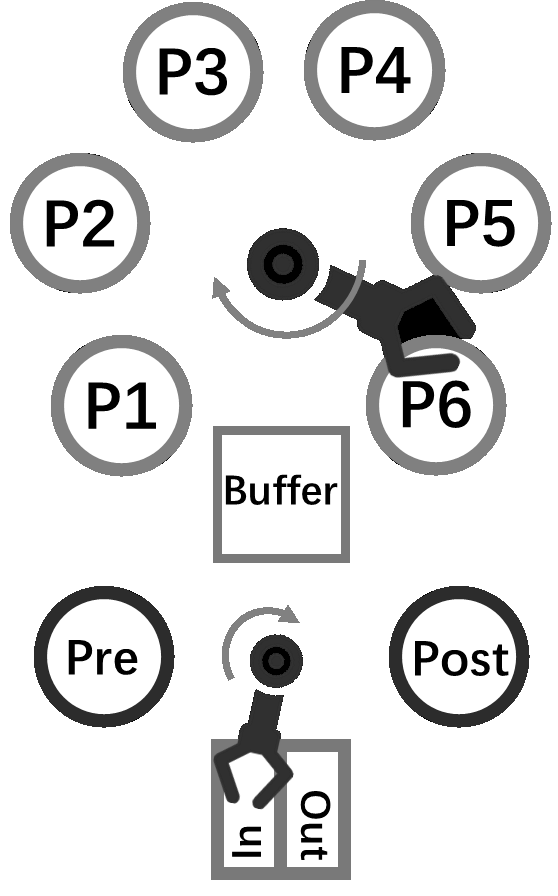
\includegraphics[width = 0.4\linewidth]{pic0.png}
            \caption{设备组合示意图}
        \end{figure}

        在图1 中,In与Out分别是产品的入口和出口,In存放待加工的产品,Out存放加工完成的产品。
        Pre与Post是产品在加工前的准备腔室和加工后的检测腔室。P1、P2、……、P6是产品的6 个加工腔室,产品将在这些不同的加工腔室中进行多种工艺的加工。
        Buffer为连接两个设备的缓冲腔室,负责两个设备间产品的传递。R1 和R2是两个机械手,负责产品在腔室加工前后的取放以及设备内的腔室之间的传递,
        其中R1可以往返于In、Out、Pre、Post和Buffer,R2可以往返于P1、P2、……、P6和Buffer。
        
        在产品加工的过程中,有时会出现多个动作需要完成,但是每个机械手每个时刻至多执行一个动作的情况。
        这些动作的执行顺序会对产品的加工时间产生很大的影响。在实际生产中,需要找到最优的机械手调度顺序,
        以使得工厂能够在最短的时间内完成产品的加工任务。
        
        显然,机械手可行的调度顺序有很多种,而课题则需要
        在其中搜索出最优的调度方案(之一)。随着工艺的增多,机械手调度的搜索空间或可行解空间会呈指数级增
        长。(这是一个NP难问题。)

        考虑如图1的设备组合,并对设备中的腔室进行如下的设定:
        
        \begin{enumerate}
        	\item 产品在腔室内的处理过程中,不需要机械手参与产品的固定、翻转或其他辅助操作
        	\item 出入口In/Out不允许存放半成品,产品的加工以及存放须严格按照其对应的工艺路径进行
        	\item 除了In/Out之外的其他腔室的容量限定为一件产品,即在任意时刻至多存放或者加工一件产品;
        	\item 产品完全放入某个腔室后,相应工艺会立即开始执行,加工结束后可以停留一段时间后再从腔室中取出;
        \end{enumerate}


        同时对每只机械手做出以下设定:
        
        \begin{enumerate}
        	\item 机械手只能顺时针旋转;
        	\item 机械手的初始位置由调度方法决定;
        	\item 机械手在任意时刻至多拿取或转移一件产品;
        	\item 机械手不能与其他机械手发生碰撞,即在Buffer腔室中不可同时对产品进行装载和卸载
        	\item 机械手从腔室中取出产品的时间为1s;
        	\item 机械手将产品放入腔室中的时间为1s;
        	\item 机械手在相邻两个腔室之间的旋转时间为1s,其中In和Out两者视为一个腔室。
        \end{enumerate}


        根据以上的设定,两只机械手将一件产品从Pre 腔室中取出并完全放入到P5腔室所需的全部时间为10s
        (R1将产品从Pre取出到放入Buffer需3s,R2将产品从Buffer取出到放入P5需7s)。

        在本课题中,每小组应对机械手调度问题进行建模,并选择自己喜欢的求解方法来解决课题设定下的三个
        问题(一种求解方法即可,多种方法以最优的一种方法计分)。每个问题的最优调度都要求总加工时间最短,并
        需要给出最优调度的总加工时间、机械手动作序列及每个动作发生的时刻、搜索算法运行时间。

		\begin{enumerate}[(a)]
			\item {求加工8件产品A 的最优调度。产品A的工艺路径及时间为
				
				A : In $\rightarrow$ Pre(60s) $\rightarrow$ Buffer $\rightarrow$ P1(240s) $\rightarrow$ P2(300s) $\rightarrow$ P3(360s) $\rightarrow$ P4(390s)$\rightarrow$ P5(270s) $\rightarrow$ P6(330s) $\rightarrow$ Buffer $\rightarrow$ Post(100s) $\rightarrow$ Out
				
				其中括号内为对应腔室所需的加工时间,Pre(60s) 表示自产品放入到Pre至允许取出需消耗60s时间。}
			\item {求加工8件产品B的最优调度。产品B的工艺路径及时间为
				
				B : In $\rightarrow$ Pre(60s) $\rightarrow$ Buffer $\rightarrow$ P1/P2(500s) $\rightarrow$ P3/P4(660s) $\rightarrow$ P5/P6(570s)$\rightarrow$ Buffer $\rightarrow$ Post(100s) $\rightarrow$ Out
				
				其中P1/P2表示P1和P2对应的工艺相同,每件产品只需进入P1或P2腔室其中之一完成加工即可。}
			\item {求加工4件产品C和4件产品D的最优调度。产品C和D的工艺路径及时间分别为
				
				C : In $\rightarrow$ Pre(60s) $\rightarrow$ Buffer $\rightarrow$ P1(180s) $\rightarrow$ P3(360s) $\rightarrow$ P5(200s)$\rightarrow$ P6(330s) $\rightarrow$ Buffer $\rightarrow$ Post(100s) $\rightarrow$ Out 
				
				D : In $\rightarrow$ Pre(60s) $\rightarrow$ Buffer $\rightarrow$ P1(180s) $\rightarrow$ P2(300s) $\rightarrow$ P4(390s) $\rightarrow$ P5(200s) $\rightarrow$ Buffer $\rightarrow$ Post(100s) $\rightarrow$ Out}
		\end{enumerate}

    }

    \subsection{符号约定}
    {
        
        首先给每个位置编号。需要注意,这里我们将buffer视为两个位置,以便让两个机械手的约束更好写。我们添加额外的约束来保证buffer处不冲突。
        \begin{table}[H]
        \centering
        \caption{位置编号}
        \begin{tabular}{@{}clc@{}}
        \toprule
        序号 & 位置 \\ \midrule
        1 & In  \\
        2 & Pre  \\
        3 & Buffer  \\
        4 & P1  \\
        5 & P2  \\
        6 & P3  \\
        7 & P4  \\
        8 & P5  \\
        9 & P6  \\
        10 & Buffer \\
        11 & Post  \\
        12 & Out  \\ \bottomrule
        \end{tabular}
        \end{table}

        定义集合 $S_1 = \{ 1, 2, 10, 11 \} $ 代表机械手1的范围,集合 $S_2 = \{ 3, 4, 5, 6, 7, 8, 9 \} $ 代表机械手2的范围。

        我们的决策变量是一个8*11的矩阵$x$,而向量$p$和矩阵$t$则是常量,含义如下:
        
        \begin{table}[H]
        \centering
        \caption{记号约定}
        \begin{tabular}{@{}clc@{}}
        \toprule
        序号 & \multicolumn{1}{c}{含义} & 符号 \\ \midrule
        1 & 将产品 $A_i$ 由位置 $j$ 取出的起始时刻     & $x(i, j)$    \\ 
        2 & 由位置 $i$ 顺时针传递到位置 $j$ 的耗时  & $t(i, j)$   \\
        3 & 产品 $A$ 在位置 $i$ 上的加工耗时   & $p(i)$ \\ \bottomrule
        \end{tabular}
        \end{table}
        备注:对于Buffer来说,位置3对应是机械手R2取出,位置10对应是机械手R1取出。$t$的取值如下:位置3等同于位置10(buffer),位置12等同于位置1(in/out)。
        \begin{figure}[H]
            \centering
            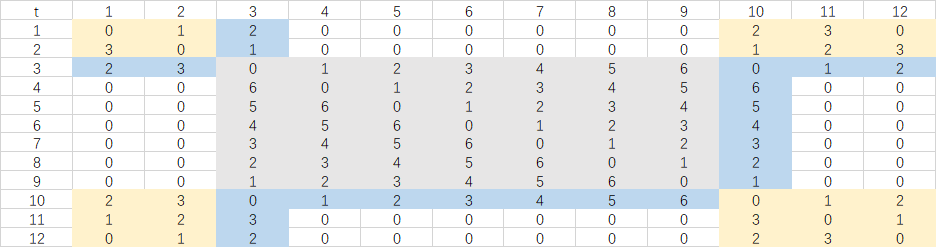
\includegraphics[width = 0.9\linewidth]{t.png}
            \caption{t的取值}
        \end{figure}

        目标函数:$$\min { \max_{i=1}^{8} { x(i, 11) } + 3}.$$

        约束条件每题各异,下文将分别说明。
            
    }

    \clearpage
}


\section{第一题}
{

    \subsection{原始优化模型}
    {
    
        \subsubsection{约束条件:}
        {
    
            (1)每个机器不能同时处理多个产品。
            区间 $$[ x(m, i) + 1 + t(i, i+1) , x(m, i+1) + 1 ]$$ 与区间 $$[ x(n, i) + 1 + t(i, i+1) , x(n, i+1) + 1 ]$$ 不能重合。这个约束对所有 $i=1, \cdots, 10$ 和 $m \neq n$ 成立。
    
            (2)Buffer 不能被两个机械手共用(位置3和位置10):
            区间 $$[ x(m, 2) + 1 + t(2, 3) , x(m, 3) + 1 ]$$ 与区间 $$[ x(n, 9) + 1 + t(9, 10) , x(n, 10) + 1 ]$$ 不能重合。这个约束对所有 $m \neq n$ 成立。
    
            (3)物体在每个位置上的处理耗时:
            $$x(n, i+1) - x(n, i) \geq 1 + p(i+1) + 1 + t(i, i+1),$$ 这个约束对所有 $n$ 成立,且对于所有的 $i=1, \cdots, 10$ 成立。
    
            (4)机械手只能顺时针转动,且一次只能取一件物体,处理完产品$m$后,需要过一段时间才能处理$n$:
            $$x(m, i) + 1 + t(i, i+1) + 1 + t(i+1, j) \leq x(n, j) \quad \mathrm{if} \quad x(m, i) \leq x(n, j),$$ 这个约束对所有的 $m \neq n$ 成立,且对于以下的 $(i, j)$ 组合成立:$i$与$j$同属$S_1$或$S_2$、$i\neq j$。
    
            (5)当$i=j$时,上面的约束演变为
            $$x(n+1, i) - x(n, i) \geq 2 + 4 + p(i),$$ 当$i \in S_1$;或
            $$x(n+1, i) - x(n, i) \geq 2 + 6 + p(i),$$ 当$i \in S_2$,其中$n=1, \cdots, 7$。
    
        }
    
        \subsubsection{等价的简化约束条件:}
        {
    
            如果我们注意到当 $m<n$ 且 $i<j$ 时,必有 $x(m, i) \leq x(n, j)$,以上的约束条件(1)(2)(4)(5)都可部分简化。
    
            (1)首先,只考虑$m<n$的情况,因为$m>n$的表达式与之重复。这样,由于$x(m, i) \leq x(n, j)$,两个区间的大小关系就确定了,区间不重合的条件等价于
            $$x(m, i+1) + 1 \leq x(m, i) + 1 + t(i, i+1)$$ 其中 $m < n$。
    
            (2)当$m<n$时,约束自然满足。当$m>n$时,区间大小关系未定。\\
            如果$x(m, 2) < x(n, 9)$,则$$x(m, 3) \leq x(n, 9) + t(9, 10)$$ 反之,$$x(n, 10) \leq x(m, 2) + t(2, 3)$$
    
            (3)不变。
    
            (4)首先,只考虑$m<n$的情况,因为$m>n$的表达式与之重复。\\
            当$m<n$且$i<j$时,由于$x(m, i) \leq x(n, j)$,两个区间的大小关系就确定了,区间不重合的条件等价于
            $$x(m, i) + 2 + t(i, i+1) + t(i+1, j) \leq x(n, j)$$
            当$m<n$且$i>j$时,两个区间的大小关系未定,区间不重合的条件等价于:如果$x(m, i) \leq x(n, j)$,则
            $$x(m, i) + 2 + t(i, i+1) + t(i+1, j) \leq x(n, j)$$ 否则
            $$x(n, j) + 2 + t(j, j+1) + t(j+1, i) \leq x(m, i)$$
    
            (5)不变。
            
             模型汇总为:
    
		    $$
		    \begin{aligned}
		    \min \quad &x(8,11)+3 \\
		    s.t. \quad &x(m, i+1) + 1 \leq x(m, i) + 1 + t(i, i+1),\quad 1\leq m < n \leq 8\quad i=1,2,\cdots,11 \\
		    \quad &x(m, 3) \leq x(n, 9) + t(9, 10) \quad \mathrm{if} \quad x(m, 2) < x(n, 9)\quad 1\leq n < m\leq 8 \\
		    \quad &x(n, 10) \leq x(m, 2) + t(2, 3) \quad \mathrm{if} \quad x(m, 2) \geq x(n, 9)\quad 1\leq n < m\leq 8 \\
		    \quad &x(n, i+1) - x(n, i) \geq 1 + p(i+1) + 1 + t(i, i+1), \quad n=1,2,\cdots,8\quad i=1,\cdots,10 \\
		    \quad &x(m, i) + 2 + t(i, i+1) + t(i+1, j) \leq x(n, j), \quad m<n \quad i<j \\
		    \quad &x(m, i) + 2 + t(i, i+1) + t(i+1, j) \leq x(n, j) \quad \mathrm{if} \quad x(m, i) \leq x(n, j), \quad m<n \quad i>j \\
		    \quad &x(n, j) + 2 + t(j, j+1) + t(j+1, i) \leq x(m, i) \quad \mathrm{if} \quad x(m, i) > x(n, j), \quad m<n \quad i>j \\
		    \quad &x(n+1, i) - x(n, i) \geq 2 + 4 + p(i), \quad n=1,\cdots,8 \quad i = 1, 2, 10, 11 \\
		    \quad &x(n+1, i) - x(n, i) \geq 2 + 6 + p(i), \quad n=1,\cdots,8 \quad i = 3, 4, 5, \cdots, 9 \\
		    \end{aligned}
		    $$
		    
        }
    
        \subsubsection{LINGO求解结果:}
        {
    
            这个结果经过了仿真程序验证。Lingo求解耗时约31秒。最优解为4890,即最后一个动作开始时刻加上3秒。
    
            \begin{figure}[H]
                \centering
                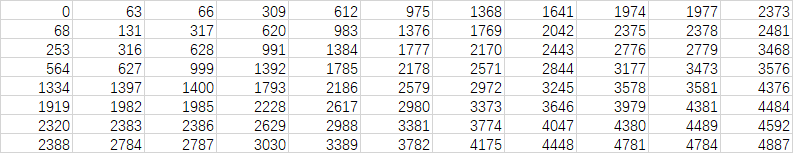
\includegraphics[width = 0.9\linewidth]{Result1.png}
                \caption{LINGO求解结果}
            \end{figure}

            \begin{figure}[H]
                \centering
                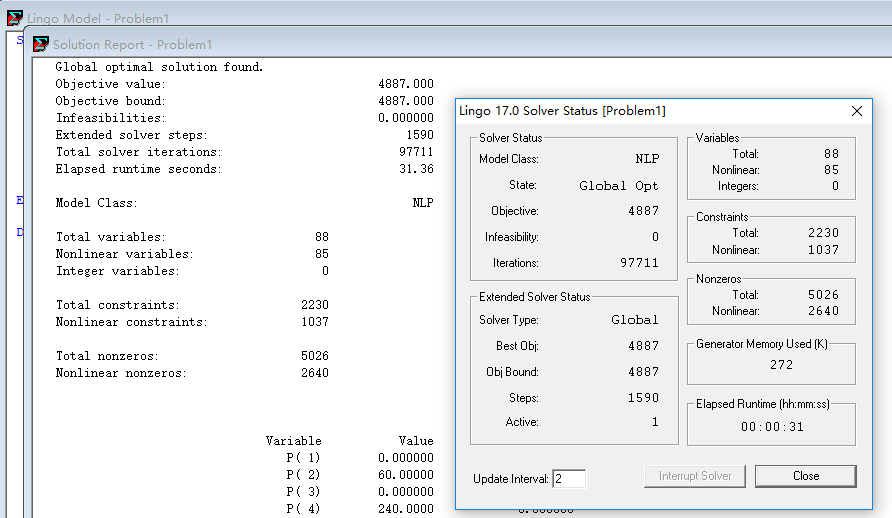
\includegraphics[width = 1\linewidth]{prob1_raw.png}
                \caption{原始模型的LINGO求解}
            \end{figure}
    
        }
        
    }

	\subsection{简化模型}

{
	
	上述的原始模型含有上千个非线性约束,Lingo求解的耗时长达31秒。虽然求解出了结果,但效率较低。
	
	为加快求解,我们考虑从以下两个方面简化模型:
	
	\begin{itemize}
		\item 考虑在一定情形下,忽略第一个机械手$R_1$,先求解$R_2$的约束,而后补充$R_1$的部分
		\item 考虑舍弃掉部分非线性约束求解子问题,而后验证舍弃的约束们是否满足。
	\end{itemize}
	
	\subsubsection{忽略第一个机械手$R_1$,直接求解$R_2$的约束}
	
	这个想法的灵感来源是我们看到了题目中给出的各个腔室加工时间分布:
	
	\begin{table}[H]
		\centering
		\caption{机械手R1涉及腔室加工时间}
		\begin{tabular}{@{}clc@{}}
			\toprule
			腔室名称 & 时间 \\ \midrule
			Pre & 60s \\
			Post & 100s  \\ \bottomrule
		\end{tabular}
	\end{table}
	
	\begin{table}[H]
		\centering
		\caption{机械手R2涉及腔室加工时间}
		\begin{tabular}{@{}clc@{}}
			\toprule
			腔室名称 & 时间 \\ \midrule
			P1 & 240s \\
			P2 & 300s \\
			P3 & 360s \\
			P4 & 390s \\
			P5 & 270s \\
			P6 & 330s  \\ \bottomrule
		\end{tabular}
	\end{table}

	看起来机械手R1涉及的腔室加工时间都小于机械手R2涉及的腔室时间,我们很自然地想到是不是在整个系统中,R2机械手的约束才是较为关键的,而R1部分可以简化甚至忽略呢?基于此思想,我们给出以下证明:
	
	\subsubsection*{证明:在本问题条件下,我们可以先求解R2再补充R1}
	
	我们需要证明,在机械手2最优解情况下,机械手1的操作由简单的加减法即可得出,而不会造成矛盾。考虑每个Buffer从物体被取出(或被放入)到下一次同样的过程的周期内($\delta \ge 0$,代表可能的时间间隔):
	
	\textbf{只有物体放入:}
	
	记两个物体放入的时间为$x_1,x_2$
	
	 \begin{table}[H]
		\centering
		\caption{只有物体放入时时刻表}
		\begin{tabular}{cc}
			\toprule
			$x_1=x_2-240-\delta$ & 物体1放入Buffer \\
			\midrule
			$x_2-66$ & 物体2取出In \\
			$x_2-63$ & 物体2放入Pre \\
			$x_2-3$ & 物体2取出Pre \\
			$x_2$ & 物体2放入Buffer \\
			\bottomrule
		\end{tabular}
	\end{table}

	\textbf{只有物体取出:}
	
	记两个物体取出的时间为$x_1,x_2$
	
	\begin{table}[H]
		\centering
		\caption{只有物体取出时时刻表}
		\begin{tabular}{cc}
			\toprule
			$x_1$ & 物体1取出Buffer  \\
			\midrule
			$x_1+3$ & 物体1放入Post  \\
			$x_1+103$ & 物体1取出Post  \\
			$x_1+106$ & 物体1放入Out \\
			$x_2=x_1+330+\delta$ & 物体2取出Post \\
			\bottomrule
		\end{tabular}
	\end{table}

	\textbf{同时有物体放入、取出:}
	
	记取出的两物体为物体6,7,放入的两物体为物体1,2
	
	\begin{table}[H]
		\centering
		\caption{只有物体取出时时刻表}
		\begin{tabular}{cc}
			\toprule
			$x$ & 物体6取出Buffer   \\
			\midrule
			$x+3$ &物体6放入Post  \\
			$x+5$ &物体1取出Pre  \\
			$x+8$ &物体1放入Buffer \\
			$x+103$ &物体6取出Post \\
			$x+106$ &物体6放入Out \\
			$x+272+\delta$ &物体2取出In \\
			$x+275+\delta$ &物体2放入Pre \\
			$x+330+\delta$ &物体7取出Buffer\\
			$x+333+\delta$ &物体7放入Post \\
			$x+335+\delta$ &物体2取出Pre  \\
			$x+338+\delta$ &物体2放入Buffer \\
			\bottomrule
		\end{tabular}
	\end{table}
	
	显然,上述经简单加减得到的过程都没有冲突。在“同时有物体放入、取出”的过程中,我们默认了物体1/2在物体6/7取出Buffer的8秒后放入Buffer(见下一章节),这可以由约束和解的最优性保证。
	
	
	\subsubsection{舍弃非线性约束,求解,再验证}
	
	为了加快模型求解速度,另一个可行的思路是求解一个子模型。考虑到在原始模型中我们有约2000个约束(其中有大约1000多个机械手非线性约束),一定会有非常多冗余没有用上的约束。这些约束使得模型求解速度变慢。
	
	事实上,由于在本题设下,机械手的运动时间都是在几秒的量级,而腔室的加工时间都是在几十甚至几百的量级,且元件前后次序较为明显。在这样的背景下忽略掉机械手的非线性约束也是容易想到的。
	
	我们在下面的的做法是求解时\textbf{忽略掉部分机械手非线性约束},待求得最优解后再验证其可行性。这种做法的正确性由以下引理保证:
	
	
	\subsubsection*{引理1:设$C$表示全部约束组成的集合,$c \subset C$,$x$是约束集$c$对应的优化问题的最优可行解,如果$x$也满足$C$中的所有约束,则$x$也是$C$对应的优化问题的最优可行解。}
	
	{
		证明:因为$x$也满足$C$中的所有约束,$x$是原问题的可行解。
		设目标函数为$\min f(x)$。假设$x$不是原问题的最优解,则存在$x'$满足$C$中的所有约束,且$f(x') < f(x)$。
		因此,$x'$满足$c$中的所有约束,从而$x'$也是约束集$c$对应的优化问题的最优可行解。
		这与“$x$是约束集$c$对应的优化问题的最优可行解”矛盾。这样,我们用反证法证明了$x$的最优性。Q.E.D.
	}
	
	\vspace{10pt}
	
	经过试验,忽略全部非线性约束(原始模型中的(2)(4)两大类约束),所得线性规划问题的最优解不满足全部的非线性约束。
	我们根据原始模型的求解经验,在全部非线性约束中,手动添加了3条。这3条是:
	(2)类约束中,只考虑元件1和6、元件2和7、元件3和8这3对约束,而忽略其余的元件对的约束。
	
	
	这样,问题就手动化为了线性规划问题,可以在0.2秒左右求解。求得的最优解,经过非线性约束的验证,确认满足全部约束条件。根据引理1,我们得到的解就是原问题的最优可行解。
	
	\subsubsection{简化后的模型表示}
	
	
	根据以上所述,我们将模型简化为如下形式:
	
	先考虑机械手2(相当于先机械原始模型中的第3列到第9列):
	
	符号约定:
	
	$$
	\begin{aligned}
	x_2(i,j)&=x(i,j+2), \quad i=1,2,3,\cdots 8, j=1,2,\cdots, 7 \\
	t_2(i,j)&=t(i,j+2), \quad i=1,2,3,\cdots 8, j=1,2,\cdots, 7 \\
	p_2(j)&=p(j+2), \quad j=1,2,\cdots, 7 \\
	\end{aligned}
	$$
	
	其中$x_2(i,j)$表示第二个机械手拿起工件的时间,$t_2(i,j)$表示第二个机械手在腔室之间的运行时间表,$p_2(j)$是第二个机械手涉及腔室的加工时间。他们和原始模型参数的关系是简单的平移。
	
	\vspace{10pt}
	
	\textbf{目标函数:}
	$$
	\min \quad x_2(8,7)
	$$
	
	\vspace{10pt}
	
	\textbf{每个机器不能同时处理多个产品:}
	$$
	x_2(m,i+1)-x_2(m+1,i) \ge 8,\quad m=1,2,3,\cdots,7, i=1,2,\cdots,6
	$$
	
	其中在只考虑一个机械手的情况下,$8=t_2(i+1,i+2)+2+t_2(i+2,i)=1+2+5$
	
	\vspace{10pt}
	
	\textbf{物体在每个位置上的处理耗时:}
	$$
	x_2(m,i+1) - x_2(m,i) \ge 3+ p_2(i+1) \quad m=1,2,3,\cdots,8, i=1,2,\cdots,6
	$$
	
	其中在只考虑一个机械手的情况下,$3=t_2(i,i+1)+2=1+2$
	
	\vspace{10pt}
	
	\textbf{解决Buffer冲突:}
	$$
	x_2(m+5,1) - x_2(m,7) \ge 11, \quad m=1,2,3
	$$
	
	其中$11=t(P6,Buffer)+2+t(Buffer,Post)+2+t(Post,Pre)+t(Pre,Buffer)+2=3+3+2+3$,解决了Buffer处的冲突。
	
	\vspace{10pt}
	
	在$x_2$平移到$x$过后,再补充机械手1的部分:
	
	$$
	\begin{aligned}
	x(n,2)&=x(n,3)-3 \\
	x(n,1)&=x(n,2)-63 \\
	x(n,10)&=x(n,9)+3 \\
	x(n,11)&=x(n,10)+103,\quad n=1,2,\cdots,8 \\
	\end{aligned}
	$$
	
	最后检查原始模型中剩下舍弃的机械手约束。
	
	模型汇总为:
	
	$$
	\begin{aligned}
	\min \quad &x_2(8,7) \\
	s.t. \quad &x_2(m,i+1)-x_2(m+1,i) \ge 8,\quad m=1,2,3,\cdots,7, i=1,2,\cdots,6 \\
	\quad &x_2(m,i+1) - x_2(m,i) \ge 3+ p_2(i+1) \quad m=1,2,3,\cdots,8, i=1,2,\cdots,6 \\
	\quad &x_2(m+5,1) - x_2(m,7) \ge 11, \quad m=1,2,3 \\
	\quad &x_2(1,1)=0, x_2(i,j) \ge 0 \\
	\end{aligned}
	$$
	
	核心机械手2线性规划部分有56个决策变量,一共有42+48+3=93个线性约束
	
	
	\subsubsection{简化模型程序运行结果}
	
	从上一部分的简化模型表示可以看出,简化后模型求解的流程如下:
	
	\begin{enumerate}
		\item 求解机械手2的模型$x_2$
		\item 将$x_2$平移到$x(:,3:9)$
		\item 补充机械手1的部分
		\item 检查模型没有用到的所有非线性约束
	\end{enumerate}
	
	程序见附录第一题部分。
	
	模型结果如下:
	
	\begin{figure}[H]
		\centering
		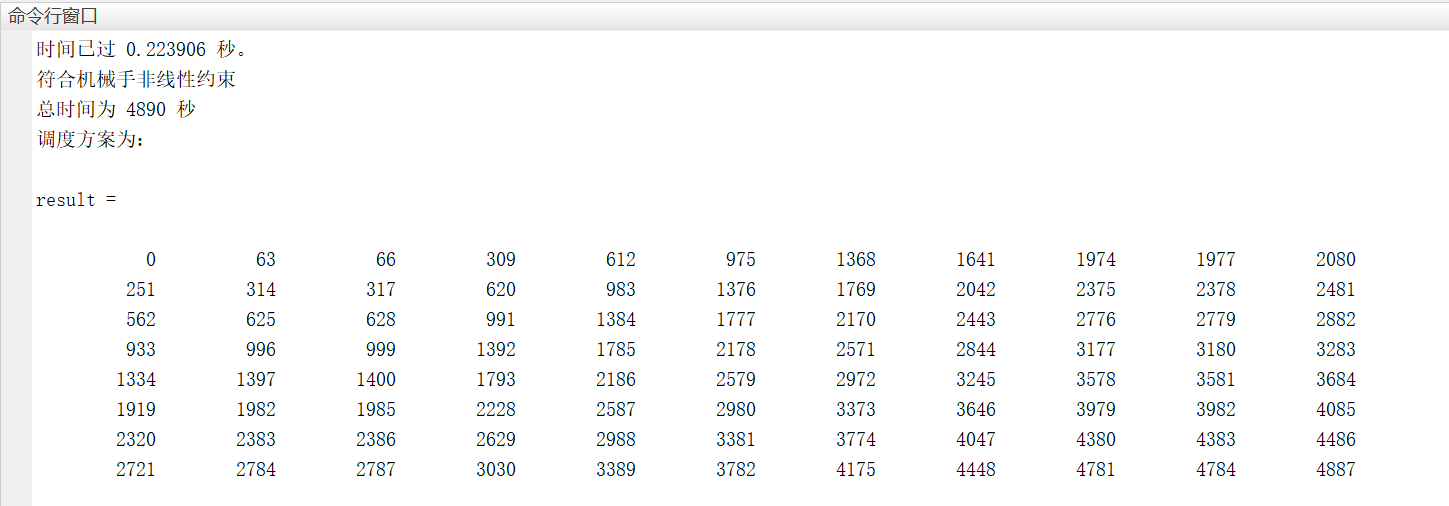
\includegraphics[width = 0.9\linewidth]{P1Result.PNG}
		\caption{简化模型MATLAB程序输出结果}
	\end{figure}
	
	可以看到模型通过了检验,即简化后得模型满足之前原始模型所有的约束。由引理1保证,我们得到的解即为最优解。
}
	
	\subsection{最优性再证明}
	{
		根据上述的讲述,我们已经可以确定我们得出的结果一定是最优解了。下面给出另一种可行的最优性证明:
		
		\begin{figure}[H]
			\centering
			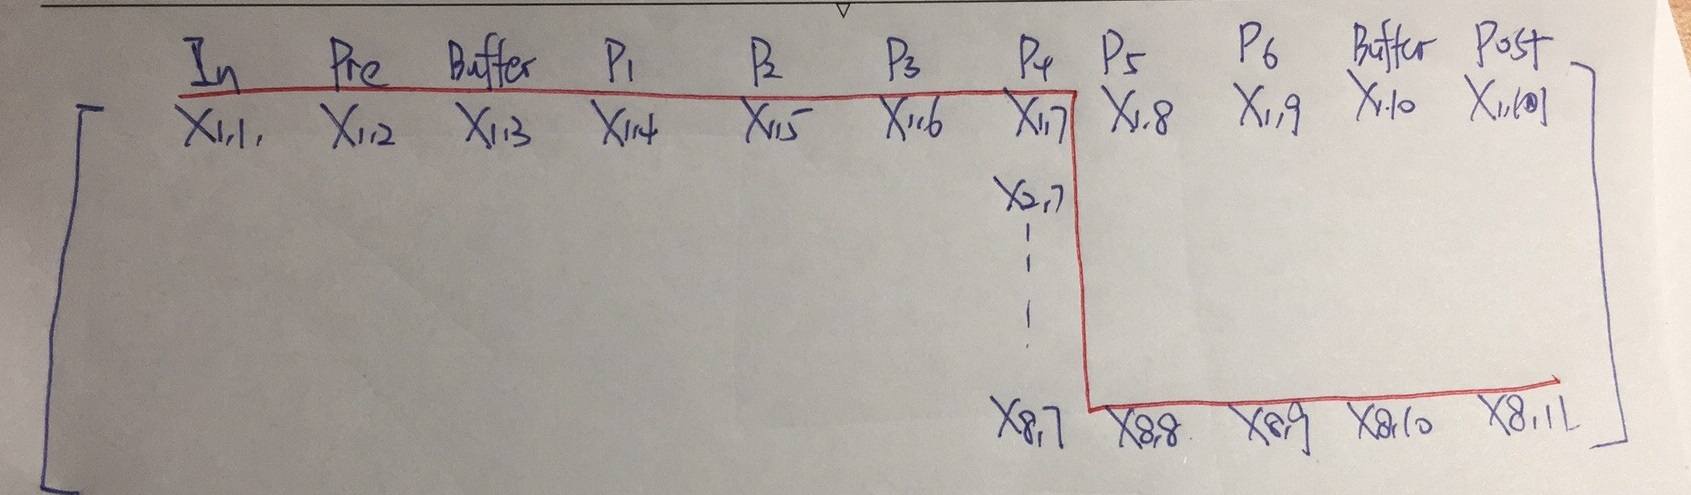
\includegraphics[width = 0.9\linewidth]{proof2.jpg}
			\caption{第一题最优性再证明:瓶颈线路图}
		\end{figure}
	
		上图是第一题的瓶颈线路图,下面我们证明这条线路图决定了最优解不小于4890:
		
		根据机械手的约束和“同一腔室不能加工两个物体”,考虑图中P4(第7列)
		$$
		\begin{aligned}
			x(8,7) &\ge x(1,7)+7(2+t(P_4,P_5)+t(P_5,P_3)+t(P_3,P_4)+p(7)) \\
			&\ge \sum_{i=1}^7 p(i)+6\times3+7\times(11+p(7))=1368+7\times 401 =4175
		\end{aligned}
		$$
		
		于是:
		$$
		x(8,11) \ge x(8,7)+ \sum_{i=8}^11 (p(i)+t(i,i+1)+2)=4175+712=4887
		$$
		
		即:
		$$
		T \ge x(8,11)+3=4890
		$$
		
		我们从另一个角度证明了第一题中最优解不小于4890. 这个结果也启示我们,最优解中这个“之字型”的每个数都是确定的。换句话说,如果这个之字型的解和我们的答案不一样的解一定不是正确的解(当然反之不然)。我们得到了一个轻松辨别解最优性的方法。
	}

    \subsection{第一题结果}
    {
		最后我们将结果转换为要求输出的结果,结果如下:

        \begin{longtable}{clc}
	
            \toprule
            序号& 机械手动作& 动作时刻\\
            \midrule 
        
        1 & R1将产品A1由In传递到Pre & 0 \\
        2 & R1将产品A1由Pre传递到Buffer & 63 \\
        3 & R2将产品A1由Buffer传递到P1 & 66 \\
        4 & R1将产品A2由In传递到Pre & 251 \\
        5 & R2将产品A1由P1传递到P2 & 309 \\
        6 & R1将产品A2由Pre传递到Buffer & 314 \\
        7 & R2将产品A2由Buffer传递到P1 & 317 \\
        8 & R1将产品A3由In传递到Pre & 562 \\
        9 & R2将产品A1由P2传递到P3 & 612 \\
        10 & R2将产品A2由P1传递到P2 & 620 \\
        11 & R1将产品A3由Pre传递到Buffer & 625 \\
        12 & R2将产品A3由Buffer传递到P1 & 628 \\
        13 & R1将产品A4由In传递到Pre & 933 \\
        14 & R2将产品A1由P3传递到P4 & 975 \\
        15 & R2将产品A2由P2传递到P3 & 983 \\
        16 & R2将产品A3由P1传递到P2 & 991 \\
        17 & R1将产品A4由Pre传递到Buffer & 996 \\
        18 & R2将产品A4由Buffer传递到P1 & 999 \\
        19 & R1将产品A5由In传递到Pre & 1334 \\
        20 & R2将产品A1由P4传递到P5 & 1368 \\
        21 & R2将产品A2由P3传递到P4 & 1376 \\
        22 & R2将产品A3由P2传递到P3 & 1384 \\
        23 & R2将产品A4由P1传递到P2 & 1392 \\
        24 & R1将产品A5由Pre传递到Buffer & 1397 \\
        25 & R2将产品A5由Buffer传递到P1 & 1400 \\
        26 & R2将产品A1由P5传递到P6 & 1641 \\
        27 & R2将产品A2由P4传递到P5 & 1769 \\
        28 & R2将产品A3由P3传递到P4 & 1777 \\
        29 & R2将产品A4由P2传递到P3 & 1785 \\
        30 & R2将产品A5由P1传递到P2 & 1793 \\
        31 & R1将产品A6由In传递到Pre & 1919 \\
        32 & R2将产品A1由P6传递到Buffer & 1974 \\
        33 & R1将产品A1由Buffer传递到Post & 1977 \\
        34 & R1将产品A6由Pre传递到Buffer & 1982 \\
        35 & R2将产品A6由Buffer传递到P1 & 1985 \\
        36 & R2将产品A2由P5传递到P6 & 2042 \\
        37 & R1将产品A1由Post传递到Out & 2080 \\
        38 & R2将产品A3由P4传递到P5 & 2170 \\
        39 & R2将产品A4由P3传递到P4 & 2178 \\
        40 & R2将产品A5由P2传递到P3 & 2186 \\
        41 & R2将产品A6由P1传递到P2 & 2228 \\
        42 & R1将产品A7由In传递到Pre & 2320 \\
        43 & R2将产品A2由P6传递到Buffer & 2375 \\
        44 & R1将产品A2由Buffer传递到Post & 2378 \\
        45 & R1将产品A7由Pre传递到Buffer & 2383 \\
        46 & R2将产品A7由Buffer传递到P1 & 2386 \\
        47 & R2将产品A3由P5传递到P6 & 2443 \\
        48 & R1将产品A2由Post传递到Out & 2481 \\
        49 & R2将产品A4由P4传递到P5 & 2571 \\
        50 & R2将产品A5由P3传递到P4 & 2579 \\
        51 & R2将产品A6由P2传递到P3 & 2587 \\
        52 & R2将产品A7由P1传递到P2 & 2629 \\
        53 & R1将产品A8由In传递到Pre & 2721 \\
        54 & R2将产品A3由P6传递到Buffer & 2776 \\
        55 & R1将产品A3由Buffer传递到Post & 2779 \\
        56 & R1将产品A8由Pre传递到Buffer & 2784 \\
        57 & R2将产品A8由Buffer传递到P1 & 2787 \\
        58 & R2将产品A4由P5传递到P6 & 2844 \\
        59 & R1将产品A3由Post传递到Out & 2882 \\
        60 & R2将产品A5由P4传递到P5 & 2972 \\
        61 & R2将产品A6由P3传递到P4 & 2980 \\
        62 & R2将产品A7由P2传递到P3 & 2988 \\
        63 & R2将产品A8由P1传递到P2 & 3030 \\
        64 & R2将产品A4由P6传递到Buffer & 3177 \\
        65 & R1将产品A4由Buffer传递到Post & 3180 \\
        66 & R2将产品A5由P5传递到P6 & 3245 \\
        67 & R1将产品A4由Post传递到Out & 3283 \\
        68 & R2将产品A6由P4传递到P5 & 3373 \\
        69 & R2将产品A7由P3传递到P4 & 3381 \\
        70 & R2将产品A8由P2传递到P3 & 3389 \\
        71 & R2将产品A5由P6传递到Buffer & 3578 \\
        72 & R1将产品A5由Buffer传递到Post & 3581 \\
        73 & R2将产品A6由P5传递到P6 & 3646 \\
        74 & R1将产品A5由Post传递到Out & 3684 \\
        75 & R2将产品A7由P4传递到P5 & 3774 \\
        76 & R2将产品A8由P3传递到P4 & 3782 \\
        77 & R2将产品A6由P6传递到Buffer & 3979 \\
        78 & R1将产品A6由Buffer传递到Post & 3982 \\
        79 & R2将产品A7由P5传递到P6 & 4047 \\
        80 & R1将产品A6由Post传递到Out & 4085 \\
        81 & R2将产品A8由P4传递到P5 & 4175 \\
        82 & R2将产品A7由P6传递到Buffer & 4380 \\
        83 & R1将产品A7由Buffer传递到Post & 4383 \\
        84 & R2将产品A8由P5传递到P6 & 4448 \\
        85 & R1将产品A7由Post传递到Out & 4486 \\
        86 & R2将产品A8由P6传递到Buffer & 4781 \\
        87 & R1将产品A8由Buffer传递到Post & 4784 \\
        88 & R1将产品A8由Post传递到Out & 4887 \\
        
            
            \bottomrule
            
            \caption{第1题的输出结果}
        \end{longtable}

        最后一个动作在4887秒的时刻开始,从Post挪动到Out,结束时刻是4890。因此,我们的最优解就是4890。
    }

    \subsection{结果讨论}
    {
    	在简化模型的时候,我们一直想到Vapnik, V.的名言:
    	
    	\begin{quotation}
    		When solving a given problem, try to avoid solving a more general problem as an intermediate step.
    	\end{quotation}
    
    	于是我们在写出庞大的初始模型后,一直在寻找本题的特殊性,寻求一种更简单的途径解决问题。幸运的是,我们找到了“R1可后算”和“机械手约束可先忽略再验证”两个可以简化的地方。这两个简化的地方来源于题目中给出的数据条件。
    	
        从最终求解结果看,绝大部分非线性约束都没有起作用,这也可以直观上得到解释:
        由于每道工序的处理时间高达几百秒,而机械手的移动耗时只有几秒,因此绝大多数情况下都是机械手空闲,等待元件处理完成。
        同样地,大部分时间内buffer处不存在两个机械手的冲突。但本题中,buffer处仍然有3处冲突,出现在第1/6元件、第2/7元件、第3/8元件处。
        我们手动将这些约束添加进约束集,实质上是如下的一种贪心算法:

        \subsubsection*{算法1:非线性约束的贪心添加算法}
        {
            \begin{outline}
                \1 第0步:将全部线性约束加入约束集$C$,忽略全部非线性约束。
                \1 第1步:求解优化问题,得到简化问题的最优解$x$。
                    \2 如果$x$满足全部约束,则$x$是原始问题的最优可行解,算法终止。
                    \2 否则,将$x$不满足的约束添加进$C$,返回第1步。
            \end{outline}

            这个算法的收敛性不能保证,但其正确性由引理1保证。
            经验上,如果初始时未加进约束集$C$的约束中,只有极少数是起作用的约束,则这种算法会很快收敛。例如,本题中,我们只手动添加了3个约束,就使该算法收敛了。
        }
    
    	另外,通过上一部分“最优性再证明”,我们可以得出所有的最优解都需要满足我们提出的“之子型”。即“之字型”上的时刻一定是确定的。
    }
    
    \clearpage
}

\section{第二题}
{
    \subsection{问题分析}
    {
        第一题的求解过程是“减约束”,即先不考虑非线性约束,在求解过程中逐步将不满足的约束添加。
        而第二题,我们采取的是“加约束”的做法。因为第二题元件的处理位置有二选一的自由度,过于灵活,我们增加以下约束,限制这种自由度,便于列写约束:

        \subsubsection*{增加约束:元件1/3/5/7走的是相同的路径,而元件2/4/6/8走的是与之互补的另一条路径。(下称“交替约束”)}

        “互补”的含义是,在$\{P_1, P_2\} $两者中的取法相反,在$\{P_3, P_4\} $两者中的取法相反,在$\{P_5, P_6\} $两者中的取法相反。
        例如,如果一条路径是“$P_1\rightarrow P_3\rightarrow P_6$”,那么与之互补的一条路径就是“$P_2\rightarrow P_4\rightarrow P_5$”。

        增加约束后,得到的解与原问题的解的关系,由以下引理给出:

        \subsubsection*{引理2:设$c$表示原问题的约束组成的集合,$c \subset C$,$x$是约束集$C$对应的优化问题的最优可行解。如果能证明在原问题的解中$x$具有最优性,则$x$也是$c$对应的优化问题的最优可行解。}

        证明显然。但关键问题是,如何证明在原问题的解中,$x$具有最优性呢?我们分3步来看。

    }

	
	

    \subsection{第一步:增加“交替”约束条件后,存在一个可行解等于4038}
    {

        我们这里假定:
        
        元件1/3/5/7走的是相同的路径:“$In\rightarrow Pre\rightarrow Buffer\rightarrow P_1\rightarrow P_3\rightarrow P_5\rightarrow Buffer \rightarrow Post \rightarrow Out$”。
        
        元件2/4/6/8走的是相同的路径:“$In\rightarrow Pre\rightarrow Buffer\rightarrow P_2\rightarrow P_4\rightarrow P_6\rightarrow Buffer \rightarrow Post \rightarrow Out$”。
        
        在这个假定下,我们用和1相似的方法提出模型(先计算机械手2再补充机械手1的部分)。
        
        \subsubsection{补充符号定义}
        {
        	$$
        	T_1=\begin{bmatrix}
        	0 & 1 & 3 & 5 \\
        	6 & 0 & 2 & 4 \\
        	4 & 5 & 0 & 2 \\
        	2 & 3 & 5 & 0 \\
        	\end{bmatrix}, T_2=\begin{bmatrix}
        	0 & 2 & 4 & 6 \\
        	5 & 0 & 2 & 4 \\
        	3 & 5 & 0 & 2 \\
        	1& 3 & 5 & 0 \\
        	\end{bmatrix}
        	$$
        	
        	其中$T_1$表示第一组(元件1/3/5/7)经过$Buffer,P1,P3,P5$时机械手2的转动时间。$T_2$表示第一组(元件2/4/6/8)经过$Buffer,P2,P4,P6$时机械手2的转动时间。
        	
        	在不同假定的分配方案下,改变的就是$T_1$和$T_2$中的值。
        }
    
    	\subsubsection{模型表示}
    	{
        
        \textbf{目标函数:}
        $$
        \min \quad x_2(8,4)
        $$
        
        \vspace{10pt}
        
        \textbf{每个机器不能同时处理多个产品:}
        $$
        \begin{aligned}
        	x_2(m,i+1)-x_2(m+2,i) &\ge 2+T_1(i+1,i+2)+T_1(i+2,i),\quad m=1,3,5, i=1,2,3 \\
        	&\ge 2+T_2(i+1,i+2)+T_2(i+2,i),  \quad m=2,4,6, i=1,2,3
        \end{aligned}
        $$
        
        \vspace{10pt}
        
        \textbf{物体在每个位置上的处理耗时:}
        $$
        \begin{aligned}
        x_2(m,i+1) - x_2(m,i) &\ge 2+T_1(i,i+1)+p_2(i+1),\quad m=1,3,5,7, i=1,2,3 \\
        &\ge 2+T_2(i,i+1)+p_2(i+1),  \quad m=2,4,6,8, i=1,2,3
        \end{aligned}
        $$
        
        \vspace{10pt}
        
        \textbf{加入机械手1带来的约束}
        $$
        x_2(m+1,1) - x_2(m,7) \ge 68, \quad m=1,2,3,\cdots,8 \\
        $$
        
        其中68是机械手1运送物件最短的间隔。$68=p(Pre)+3+3+t(Buffer,In)=60+3+3+2$
        
        \vspace{10pt}
        
        \textbf{解决Buffer冲突:}
        $$
        x_2(7,1) \ge x_2(1,4)+114
        $$
        
        其中$114=p(Post)+3+t(P5,Buffer)+2+t(Post,Out)+2+t(Post,Pre)+t(Buffer,Post)$,解决了Buffer处的冲突。
        }
    
    	在求解出$x_2$后,我们平移至$x$,而后补充机械手1部分:
    	
    	$$
    	\begin{aligned}
    	x(n,2)&=x(n,3)-3 \\
    	x(n,1)&=x(n,2)-63 \\
    	x(n,10)&=x(n,9)+3 \\
    	x(n,11)&=x(n,10)+103,\quad n=1,2,\cdots,8 \\
    	\end{aligned}
    	$$
    	
    	最后检查原始模型中剩下舍弃的机械手约束。
    
    	模型表示汇总如下:
    	
		$$
		\begin{aligned}
		\min \quad &x_2(8,4) \\
		s.t. \quad &x_2(m,i+1)-x_2(m+2,i) \ge \begin{cases}
		2+T_1(i+1,i+2)+T_1(i+2,i) &m=1,3,5,7\\
		2+T_2(i+1,i+2)+T_2(i+2,i) &m=2,4,6,8
		\end{cases}, i=1,2,3 \\
		\quad &x_2(m,i+1) - x_2(m,i) \ge  \begin{cases}
		2+T_1(i,i+1)+p_2(i+1) &m=1,3,5,7\\
		2+T_2(i,i+1)+p_2(i+1) &m=2,4,6,8
		\end{cases}, i=1,2,3 \\
		\quad &x_2(m+1,1) - x_2(m,7) \ge 68, \quad m=1,2,3,\cdots,8 \\
		\quad &x_2(7,1) \ge x_2(1,4)+114 \\
		\quad &x_2(1,1)=0, x_2(i,j) \ge 0 \\
		\end{aligned}
		$$
		
		一共有32个决策变量,51个线性约束。有1000多个非线性约束需要检验。

		\subsubsection{模型的求解}
		{
			和第一题类似的方法,我们编写了MATLAB程序求解上述线性规划问题。模型的流程和第一题一样。
			
			模型的代码见附录部分。
			
			程序运行结果如下:
			
			\begin{figure}[H]
				\centering
				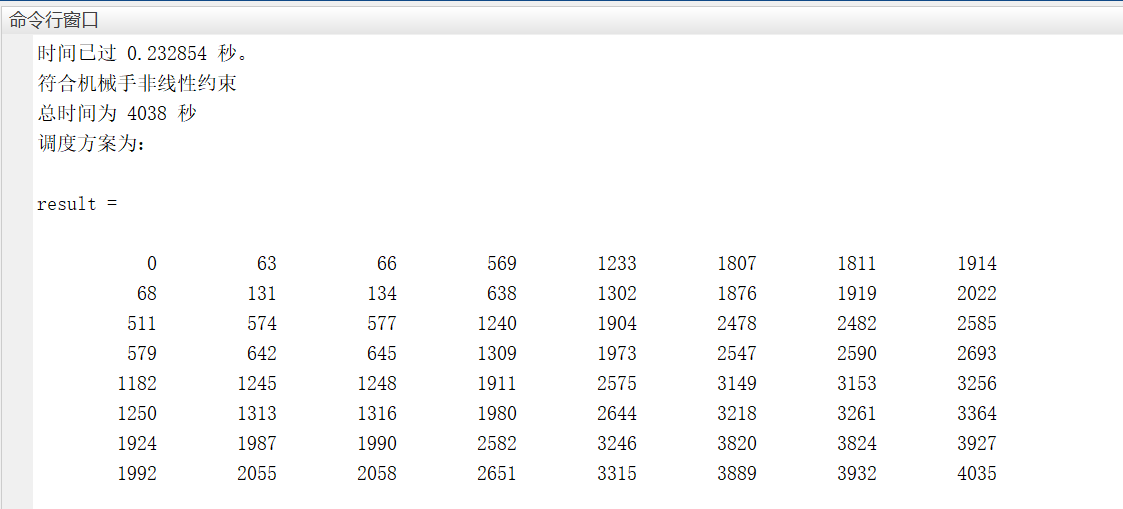
\includegraphics[width = 0.9\linewidth]{P2Result.PNG}
				\caption{在特定分配下,一个4038的可行解}
			\end{figure}
		
			得出结果后进行了机械手约束检查。第二题的机械手检查编写比第一题难一些(下一个房间不再是简单的+1关系,而需要额外判断)。但思路上和第一题一模一样。
			
			后面我们将证明,我们得出的解就是第二题的最优解。
		}
		
      
    }

    \subsection{第二步:增加“交替”约束条件后,最优解一定不小于4038}
    {
        我们这里放宽第一步的限制。虽然仍然假设元件1/3/5/7和元件2/4/6/8 分别走相同的路径,但路径本身不需要指定。
        
        整个证明的遵循着以下的线路:
        
        \begin{figure}[H]
        	\centering
        	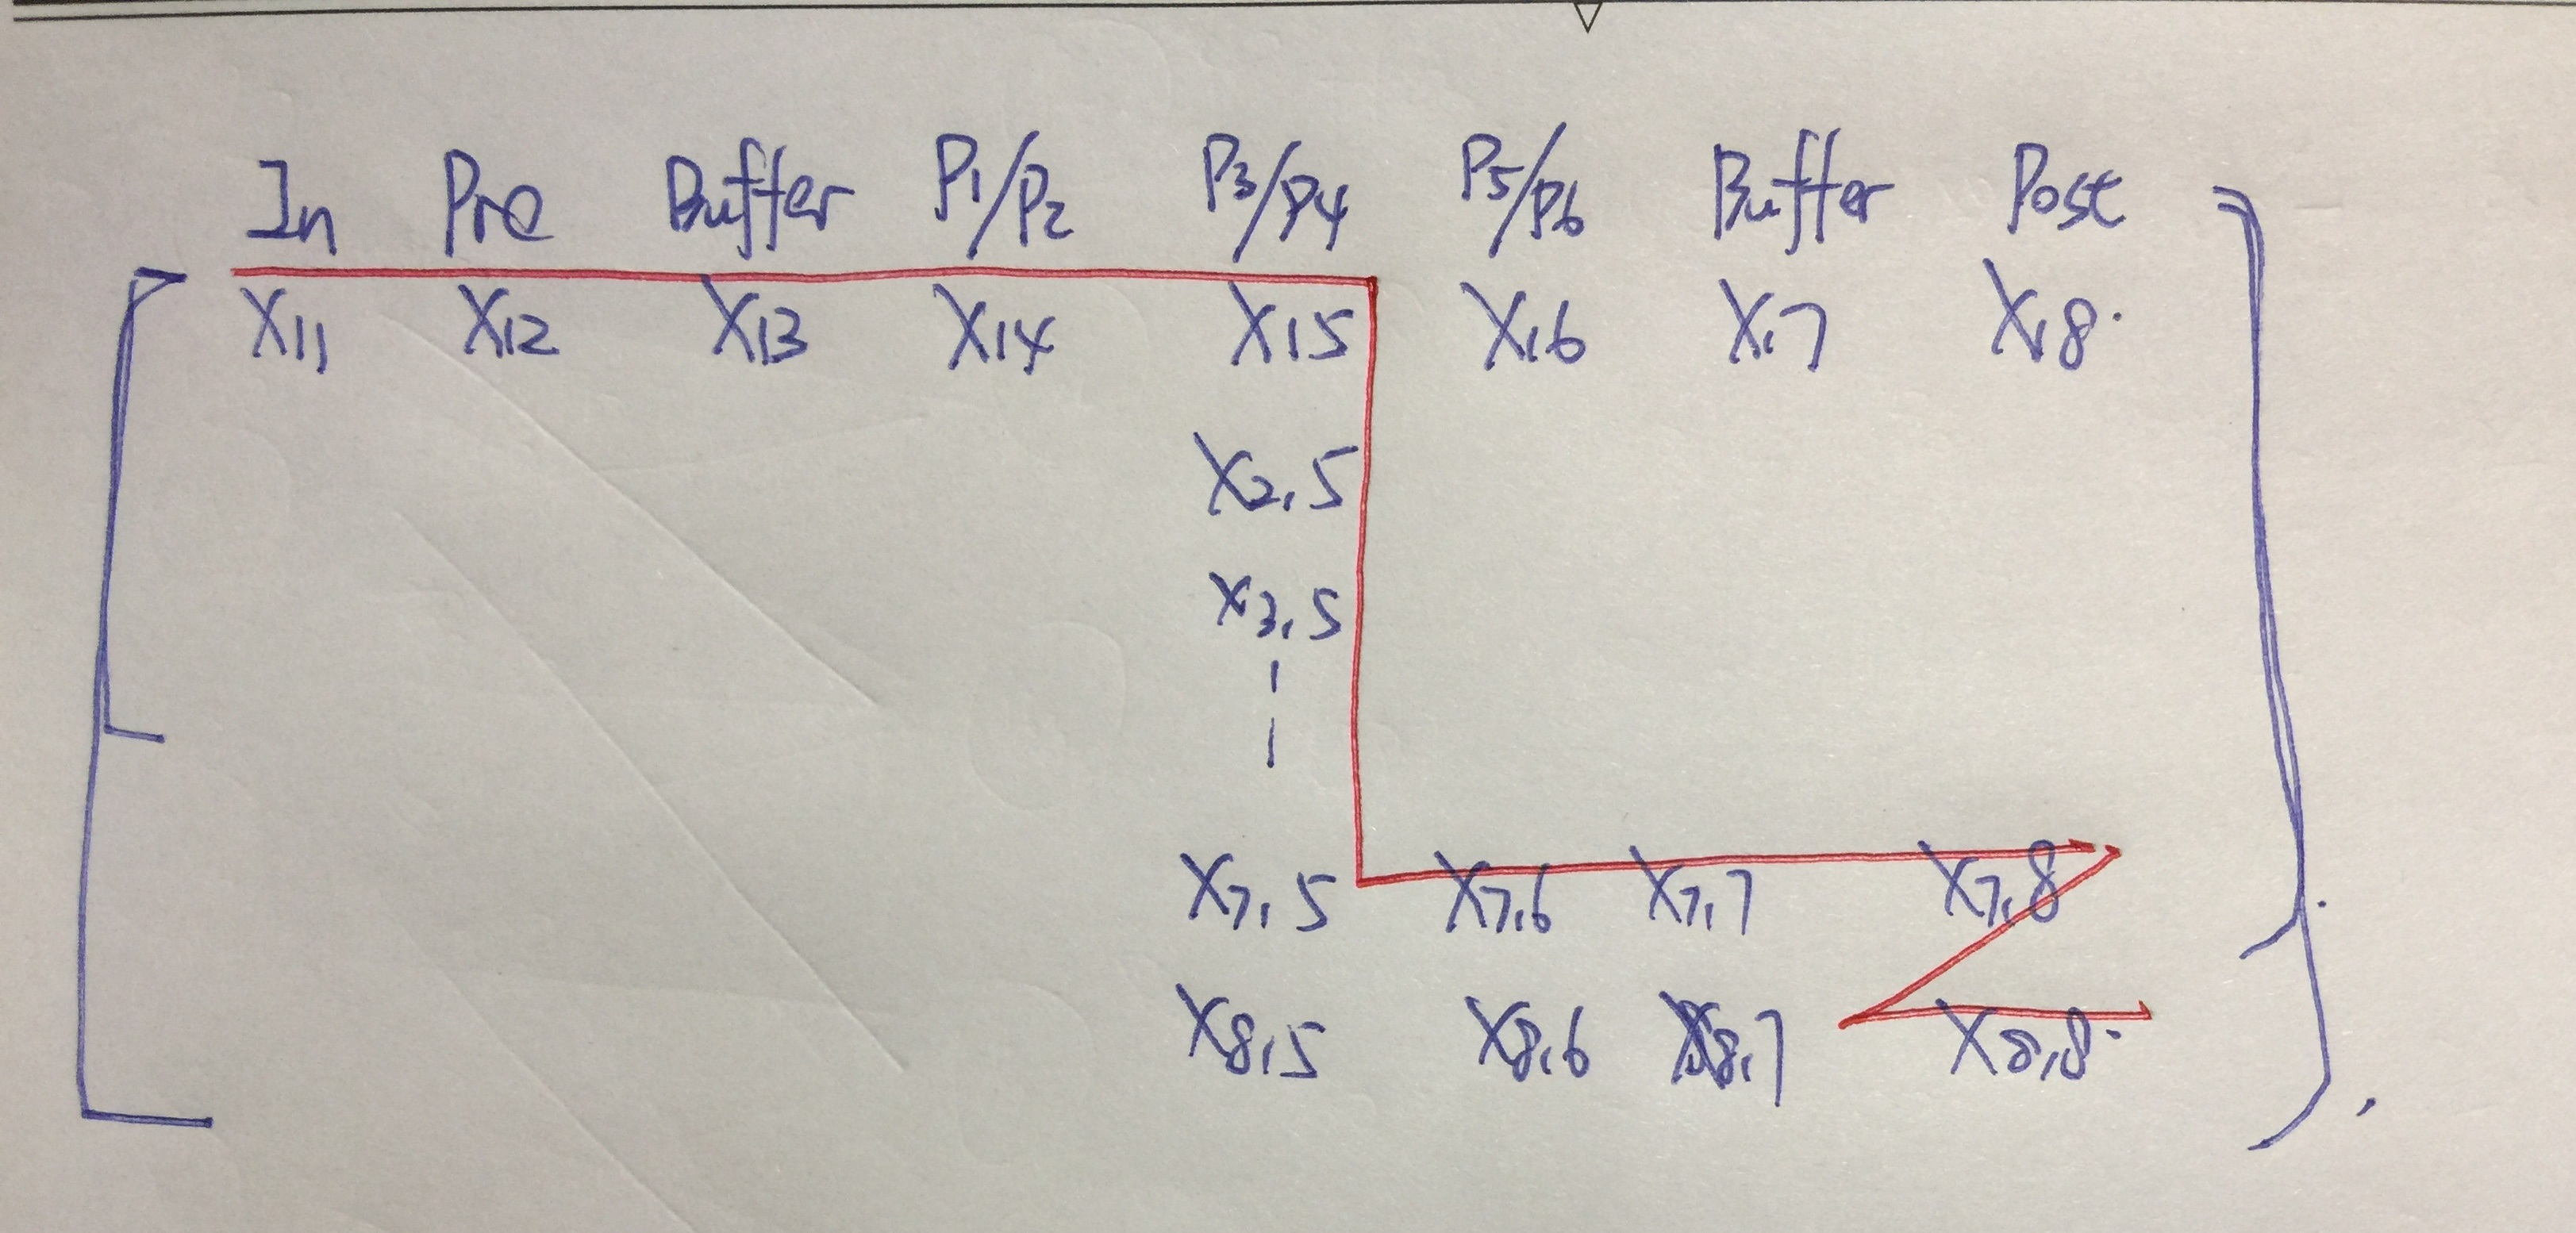
\includegraphics[width = 0.9\linewidth]{proof1.jpg}
        	\caption{增加“交替”约束条件后,最优解一定不小于4038,瓶颈线路图}
        \end{figure}
        
        假设元件1/3/5/7进入$x_1,x_2,x_3$号腔室,元件2/4/6/8进入$y_1,y_2,y_3$号腔室。其中$x_1,y_1 \in \{P_1,P_2\},x_1 \neq y_1$,$x_2,y_2 \in \{P_3,P_4\},x_2 \neq y_2$,$x_3,y_3 \in \{P_5,P_6\},x_3 \neq y_3$。
        
        考虑$P_3/P_4$,即$x_2$中的第三个腔室,$x$中的第五个腔室。根据约束的关系:
		
		$$
		\begin{aligned}
		x(7,5) &\ge x(1,5)+3[t(x_2,x_3)+t(x_3,x_1)+t(x_1,x_2)+4+p(5)] \\
		&=x(1,5)+3 \times 671
		\end{aligned}
		$$
		
		而$$
		x(1,5) \ge \sum_{i=1}^5 p(i)+6+2+2+t(Buffer,x_1)+t(x_1,x_2)=1230+t(buffer,x_2)
		$$
		
		于是$$
		x(7,5) \ge 3243+t(Buffer,x_2) 
		$$
		
		进一步:
		
		$$
		\begin{aligned}
		x(7,8) &\ge x(7,5)+t(x_2,x_3)+t(x_3,Buffer)+2+2+p(6)+p(Post)+3 \\
		&\ge 3920+t(x_2,x_3)+t(x_3,Buffer)+t(Buffer,x_2)=3920+7=3927
		\end{aligned}
		$$
		
		于是:
		$$
		x(8,8) \ge x(7,8)+t(8,1)+2+t(1,Buffer)+p(Post)+3=x(7,8)+108=3927+108=4035
		$$
		
		即:
		$$
		T \ge x(8,8)+3 = 4038
		$$
		

		
    }

    \subsection{第三步:不满足这个“交替”约束条件后,最优解一定不小于4038}
    {
    	在第三步的证明中,由于要考虑不满足“交替”的条件,之间$8 \times 8$的矩阵形式不能推广了。我们重新回到第一题的形式,即:
    	
    	\begin{figure}[H]
    		\centering
    		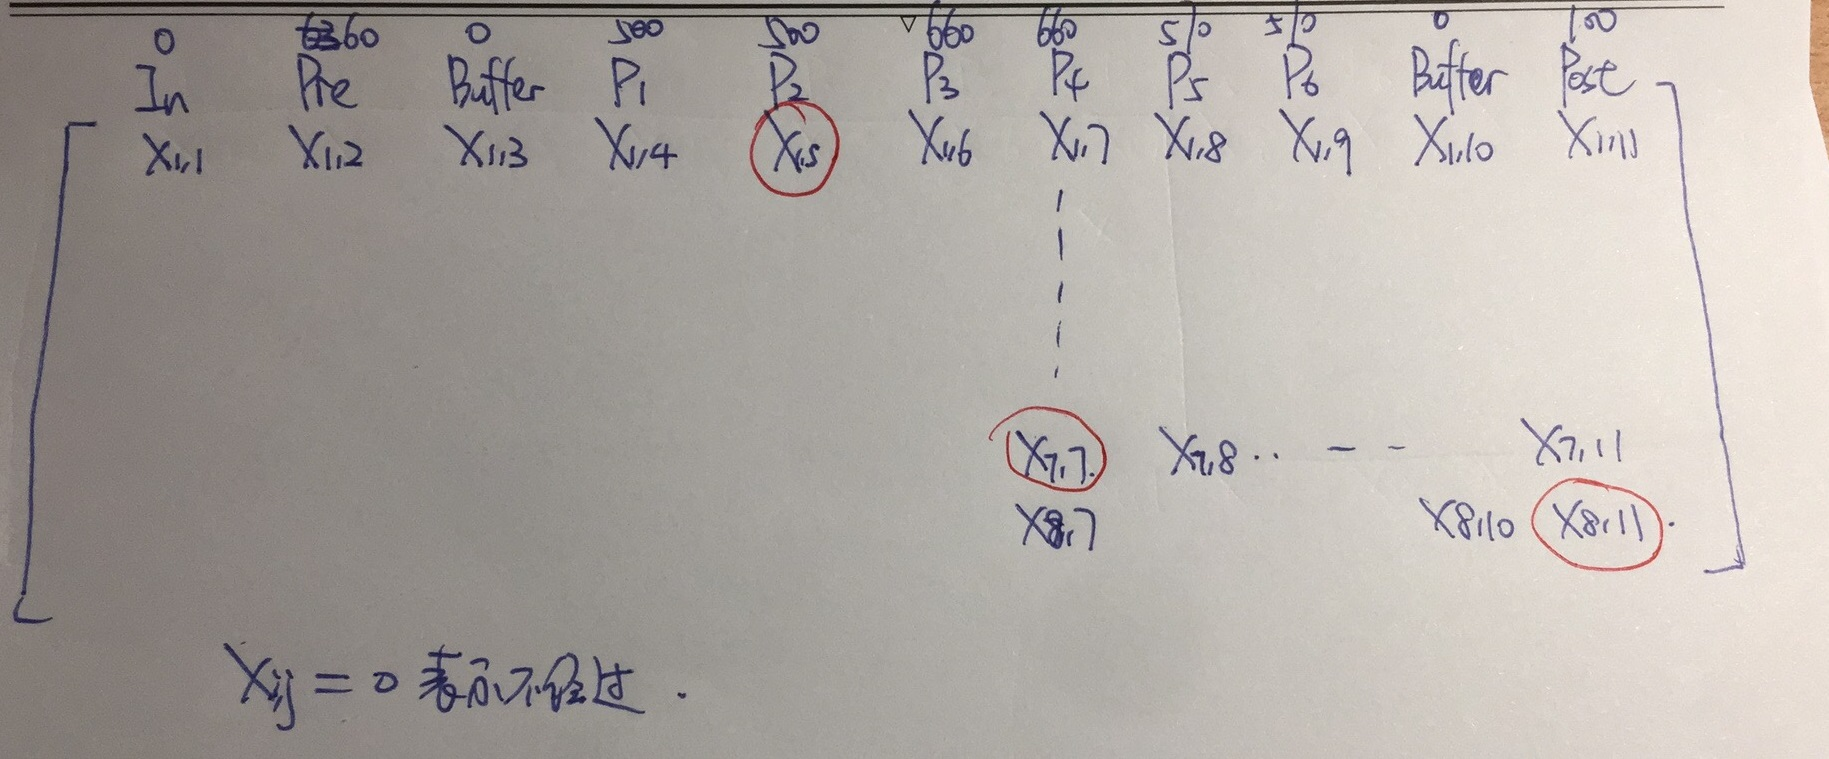
\includegraphics[width = 0.9\linewidth]{proof3.jpg}
    		\caption{第三步证明中的参数表示(重新回到$8 \times 11$)}
    	\end{figure}
    	
    	我们下面要证明的是$x(8,11)$和$x(7,7)$有一定的先后关系,而在任意情况下$x(7,7) \ge 3247$。
    	
    	
        记
        
        $$
        \begin{aligned}
        x(1, 5)=x(1,4)+1&\ \quad if \  x(1,5)=0\\
        x(7, 7)=x(7,6)+1&\ \quad if\ x(7,7)=0
        \end{aligned}
        $$
        
        则根据约束,有
        
        $$
        \begin{aligned}
        x(1,5)&\ge570\\
        x(8,11)+3-x(7,7)&\ge891
        \end{aligned}
        $$
        
        假设有“交替”约束,则
        
        $$
        x(7, 7)-x(1, 5)\ge2677
        $$
        
        从而
        
        $$
        x(8,11)+3\ge4038
        $$
        
        因此我们需要证明
        
        \begin{equation}\label{equ:square} 
        	x(7,7)\ge3247
        \end{equation}
        
        
        \textbf{引理3}
        
        $$
        x(m,6)-x(n,6)\ge671\ (m>n, x(m,6),x(n,6)\neq0) 
        $$
        
        记$y(m,n)$为第$m$个物体从第$n$个位置离开的时间,则
        
        $$
        x(n,6)\ge y(n,6)+660\ge x(n,5)+663\ge y(m,8)+667 \ge x(m,6)-671
        $$
        
        引理得证。
        该引理显然对$x(m,7)-x(n,7)$同样成立。
        
        因此:
        
        \begin{enumerate}[(i)]
        	\item 当物体$1-7$中有5个或以上经过位置6或7时,(\ref{equ:square})成立
        	这是由于
        	
        	$$
        	x(7,7)\ge 671*4+x(1,6)\ge 671*4+660+x(1,5)\ge 671*4+660+570=3914
        	$$
        	\item 假设物体1经过位置6,则物体$1-7$中有4个经过位置7时。(\ref{equ:square})成立
        	假设物体m第一个经过位置7,则
        	
        	$$
        	x(7,7)\ge 671*3+x(m,7)\ge 671*3+660+x(m,5)\ge 671*3+660+570+68=3311
        	$$
        	
        	因此,取最优解时一定有4个物体经过物体1经过的位置6(或7)。此时
        	
        	$$
        	x(7, 7)-x(1, 5)\ge 671*4+660+4=2677
        	$$
  
        	成立。
        \end{enumerate}
    
        由(i),(ii)可知(\ref{equ:square})成立。Q.E.D.
        
    }

    \subsection{第二题结果}
    {
        从逻辑上说,以上3个小节的结论,已经能充分证明4038这个解的最优性。由于它是增加“交替”约束条件后的最优可行解,根据引理2,它就是原问题的最优可行解(之一)。

        我们的程序输出的机械手的动作序列如下:

        \begin{longtable}{clc}
	
            \toprule
            序号& 机械手动作& 动作时刻\\
            \midrule 
            
        1 & R1将产品B1由In传递到Pre & 0 \\
        2 & R1将产品B1由Pre传递到Buffer & 63 \\
        3 & R2将产品B1由Buffer传递到P1 & 66 \\
        4 & R1将产品B2由In传递到Pre & 68 \\
        5 & R1将产品B2由Pre传递到Buffer & 131 \\
        6 & R2将产品B2由Buffer传递到P1 & 134 \\
        7 & R1将产品B3由In传递到Pre & 511 \\
        8 & R2将产品B1由P1传递到P3 & 569 \\
        9 & R1将产品B3由Pre传递到Buffer & 574 \\
        10 & R2将产品B3由Buffer传递到P1 & 577 \\
        11 & R1将产品B4由In传递到Pre & 579 \\
        12 & R2将产品B2由P2传递到P4 & 638 \\
        13 & R1将产品B4由Pre传递到Buffer & 642 \\
        14 & R2将产品B4由Buffer传递到P1 & 645 \\
        15 & R1将产品B5由In传递到Pre & 1182 \\
        16 & R2将产品B1由P3传递到P5 & 1233 \\
        17 & R2将产品B3由P1传递到P3 & 1240 \\
        18 & R1将产品B5由Pre传递到Buffer & 1245 \\
        19 & R2将产品B5由Buffer传递到P1 & 1248 \\
        20 & R1将产品B6由In传递到Pre & 1250 \\
        21 & R2将产品B2由P4传递到P6 & 1302 \\
        22 & R2将产品B4由P2传递到P4 & 1309 \\
        23 & R1将产品B6由Pre传递到Buffer & 1313 \\
        24 & R2将产品B6由Buffer传递到P1 & 1316 \\
        25 & R2将产品B1由P5传递到Buffer & 1807 \\
        26 & R1将产品B1由Buffer传递到Post & 1811 \\
        27 & R2将产品B2由P6传递到Buffer & 1876 \\
        28 & R2将产品B3由P3传递到P5 & 1904 \\
        29 & R2将产品B5由P1传递到P3 & 1911 \\
        30 & R1将产品B1由Post传递到Out & 1914 \\
        31 & R1将产品B2由Buffer传递到Post & 1919 \\
        32 & R1将产品B7由In传递到Pre & 1924 \\
        33 & R2将产品B4由P4传递到P6 & 1973 \\
        34 & R2将产品B6由P2传递到P4 & 1980 \\
        35 & R1将产品B7由Pre传递到Buffer & 1987 \\
        36 & R2将产品B7由Buffer传递到P1 & 1990 \\
        37 & R1将产品B8由In传递到Pre & 1992 \\
        38 & R1将产品B2由Post传递到Out & 2022 \\
        39 & R1将产品B8由Pre传递到Buffer & 2055 \\
        40 & R2将产品B8由Buffer传递到P1 & 2058 \\
        41 & R2将产品B3由P5传递到Buffer & 2478 \\
        42 & R1将产品B3由Buffer传递到Post & 2482 \\
        43 & R2将产品B4由P6传递到Buffer & 2547 \\
        44 & R2将产品B5由P3传递到P5 & 2575 \\
        45 & R2将产品B7由P1传递到P3 & 2582 \\
        46 & R1将产品B3由Post传递到Out & 2585 \\
        47 & R1将产品B4由Buffer传递到Post & 2590 \\
        48 & R2将产品B6由P4传递到P6 & 2644 \\
        49 & R2将产品B8由P2传递到P4 & 2651 \\
        50 & R1将产品B4由Post传递到Out & 2693 \\
        51 & R2将产品B5由P5传递到Buffer & 3149 \\
        52 & R1将产品B5由Buffer传递到Post & 3153 \\
        53 & R2将产品B6由P6传递到Buffer & 3218 \\
        54 & R2将产品B7由P3传递到P5 & 3246 \\
        55 & R1将产品B5由Post传递到Out & 3256 \\
        56 & R1将产品B6由Buffer传递到Post & 3261 \\
        57 & R2将产品B8由P4传递到P6 & 3315 \\
        58 & R1将产品B6由Post传递到Out & 3364 \\
        59 & R2将产品B7由P5传递到Buffer & 3820 \\
        60 & R1将产品B7由Buffer传递到Post & 3824 \\
        61 & R2将产品B8由P6传递到Buffer & 3889 \\
        62 & R1将产品B7由Post传递到Out & 3927 \\
        63 & R1将产品B8由Buffer传递到Post & 3932 \\
        64 & R1将产品B8由Post传递到Out & 4035 \\
            
            
            \bottomrule
            
            \caption{第2题输出结果}
        \end{longtable}

        最后一个动作在4035秒的时刻开始,从Post挪动到Out,结束时刻是4038。因此,我们的最优解就是4038。
    }
	
	\subsection{结果讨论}
	{
		在第二题的求解过程中我们采取了“三步走”的策略。事实上“三步走”策略是一种王焕钢老师提倡的“从特殊到一般”的过程。
		
		我们先通过直觉加上一个很强的“交替”条件。增加这个“交替”条件的灵感来自于实际。实际中由于腔室的可替代性,人在做的时候很容易将元件分成两组“并行”通过。“交替”条件的灵感来源于此。
		
		我们只求解了一种最特殊的情况(指定了通过路线)。第二步的证明告诉我们其他七种(一共2*2*2=8种并行策略)的最优解都大于等于4038,而第三步在第二步的基础上验证了我们的直觉“并行”的最优性。
		
		这是一个很好的“从猜想到验证的过程”。
	}

	

    \clearpage
}

\section{第三题}
{
    \subsection{问题分析}
    {
        第三问的难点在于,元件有C、D两种,且进入顺序是未知的。8个元件分为2种,每种4个,则排列顺序有70种,如果遍历的话复杂度太高。

        因此,我们对第一题中的约束条件做了如下修改:
        \begin{itemize}
            \item 不再规定下标小的元件一定先进入,元件的进入次序是任意的。
        \end{itemize}

        这样,第一题的5大类约束中,第1类约束(与位置有关)就由线性变为了非线性,因为不再能假定元件遵循下标次序进入。
        同时,其他的约束中出现的常量$t$和$p$,也要根据元件的具体类型,做相应修改。
		
    }

    \subsection{原始优化模型}
    {
        和第一题类似,我们先写出原始优化模型,既有线性约束,也有非线性约束。

        \subsubsection{补充符号定义}
        {
        	由于第三题的复杂性,为讨论方便,第三题的记号作以下补充:
        	\begin{table}[H]
        		\centering
        		\caption{第三题符号约定}
        		\begin{tabular}{@{}clc@{}}
        			\toprule
        			序号 & \multicolumn{1}{c}{含义} & 符号 \\ \midrule
        			1 & 将产品 $i$ 由位置 $j$ 取出的起始时刻     & $x(i, j)$    \\ 
        			2 & 将产品 $i$ 放入位置 $j$ 的终止时刻     & $y(i, j)$    \\ 
        			3 & 由位置 $i$ 顺时针传递到位置 $j$ 的耗时  & $t(i, j)$   \\
        			4 & 产品 $C$ 在位置 $i$ 上的加工耗时   & $p(1,i)$ \\
        			5 & 产品 $D$ 在位置 $i$ 上的加工耗时   & $p(2,i)$ \\
        			6 & 第 $j$ 个进入的产品 $C$ 的编号 $i$  & $P(1,j)$ \\
        			7 & 第 $j$ 个进入的产品 $D$ 的编号 $i$  & $P(2,j)$ \\
        			8 & 产品 $C$ 经过各位置的顺序  & $S(1,j)$ \\ 
        			9 & 产品 $D$ 经过各位置的顺序  & $S(2,j)$ \\ \bottomrule
        		\end{tabular}
        	\end{table}
        	
        	上述记号中,$x$和$y$是决策变量,而其余为常量。
        	
        	$t(i, j)$的取值与第一题相同。
        	
        	$P(i,j)$ 的取值如下:
        	
        	\begin{figure}[H]
        		\centering
        		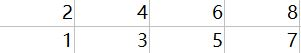
\includegraphics[width = 0.6\linewidth]{pij3.jpg}
        		\caption{$P(i,j)取值$}
        	\end{figure}
        
        	这样的取值主要是为了简化模型的方便。对原始模型,不同的取值意义是相同的。
        }
    
    	\subsubsection{模型表示}
    	{
    		\textbf{目标函数:}
    		$$\min { \max_{i=1}^{8} { y(i, 12) } }.$$
    		
    		\textbf{机械手运动时间约束}
    		$$
    		\begin{aligned}
    		x(P(1,m),S(1,i))+t(S(1,i),S(1,i+1))&=y(P(1,m),S(1,i+1))\\
    		x(P(2,m),S(2,i))+t(S(2,i),S(2,i+1))&=y(P(2,m),S(2,i+1))
    		\end{aligned}
    		$$
    		
    		\textbf{每个机器不能同时处理多个产品:}
    		
    		$$
    		[y(m,i)-1,x(m,i)+1]
    		$$
    		
    		与
    		
    		$$
    		[y(n,i)-1,x(n,i)+1]
    		$$
    		
    		不重合。这个约束对$\{(i,j) | i\in P(k,:), j\in S(k,:), j\neq 1\ nor\ 12\}$,且$m\neq n$成立。
    		
    		\textbf{Buffer 不能被两个机械手共用(位置3 和位置10):同2.1.1(2)}
    		
    		区间 $$[ y(m,3)-1 , x(m, 3) + 1 ]$$ 与区间 $$[ y(n,10)-1 , x(n, 10) + 1 ]$$ 不能重合。这个约束对所有 $m \neq n$ 成立。
    		
    		\textbf{物体在每个位置上的处理耗时:}
    		
    		 $$x(n, i) \geq p(k,i) + x(n, i) ,$$ 这个约束对所有 $n\in P(k_2,:)$成立,且对于所有的 $i=1, \cdots, 10$ 成立。
    		 
    		 \textbf{机械手只能顺时针转动,且一次只能取一件物体,处理完产品$m$后,需要过一段时间才能处理$n$:}
    		 
			 $$y(m, S(k_1,i+1))+ t(S(k_1,i+1), S(k_2,j)) \leq x(n, S(k_2,j)) \quad \mathrm{if} \quad y(m, S(k_1,i+1) \leq S(k_2,j+1),$$ 这个约束对所有的 $m \neq n$ 成立,且对于以下的 $(S(k_1,i), S(k_2,j))$ 组合成立:同属$S_1$或$S_2$、$S(k_1,i)\neq S(k_2,j)$、$m\in P(k_1,:), n\in P(k_2,:)$。
    	}
    }

    \subsection{简化模型}
    {
		由于以上模型非线性约束过于复杂,使用LINGO运行时间过长,我们将对以上约束进行减弱以增快运行速度。
		
		对于上述(1-4)约束,虽然有一定的简化空间,但考虑到模型的泛化能力我们不进行简化。
		
		对于约束(5),即机械手约束:

		在机械手1的约束中,我们注意到:
		当 $m<n, m, n\in S1$ 且 $i<j$ 时,有 $x(m, i) \leq x(n, j)$。此时,两个区间的大小关系就确定了,区间不重合的条件等价于
		
		$$
		y(m, i+1) + t(i+1, j) \leq x(n, j)
		$$
		
		当$m<n$且$i>j$时,两个区间的大小关系未定,区间不重合的条件等价于:如果$x(m, i) \leq x(n, j)$,则
		$$x(m, i) + 2 + t(i, i+1) + t(i+1, j) \leq x(n, j)$$ 否则
		$$x(n, j) + 2 + t(j, j+1) + t(j+1, i) \leq x(m, i)$$
		
		在机械手2的约束中,上述简化不易进行。这是因为即使预先按各物体进入的顺序排列,也不能保证上述大小关系成立。然而,保留所有机械手2的约束会使程序运行时间无法忍受。因此,我们效仿2.2.2的做法,舍弃大部分机械手2的约束。我们根据原始模型的求解经验,在舍去机械手2全部非线性约束中,添加了5条:
		
		$$
		\begin{aligned}
		x(P2(m), 7) + 7 &\le x(P2(m+1), 5);\\
		x(P2(m), 5) + 8 &\le x(P2(m+1), 4);\\
		x(P2(m), 8) + 7 &\le x(P1(m+1), 6);\\
		x(P1(m), 6) + 7 &\le x(P1(m+1), 4);\\
		x(P1(m), 9) + 8 &\le x(P1(m+1), 8);\\
		m&=1,2,3;
		\end{aligned}
		$$
		
		这样,问题就手动化为了较简单的线性规划问题。求得的最优解,经过非线性约束的验证,确认满足全部约束条件。根据LINGO对原始约束模型的部分约束的求解,减弱版的解和原解下界相同。因此,我们得到的解就是原问题的最优可行解。
        
    }

	\subsection{程序运行结果}
	{
		这个结果经过了仿真程序验证。Lingo求解耗时约45秒。最优解为2716(这里目标函数加上了3)。
		
		\begin{figure}[H]
			\centering
			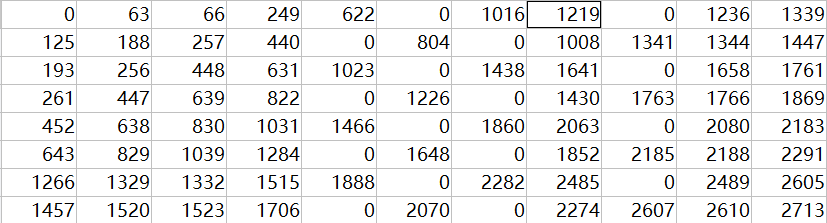
\includegraphics[width = 0.9\linewidth]{Result3.png}
			\caption{LINGO求解结果}
		\end{figure}
		
		\begin{figure}[H]
			\centering
			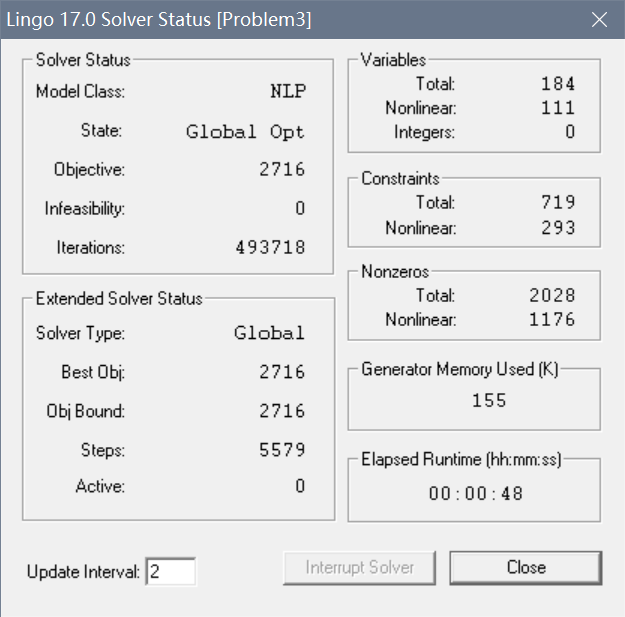
\includegraphics[width = 0.7\linewidth]{prob3_raw.png}
			\caption{LINGO求解结果}
		\end{figure}
			
	}

    \subsection{第三题结果}
    {
        我们的程序输出的机械手的动作序列如下:
        
          \begin{longtable}{clc}
        	
        	\toprule
        	序号& 机械手动作& 动作时刻\\
        	\midrule 
        	
1 & R1将产品D1由In传递到Pre & 0 \\
2 & R1将产品D1由Pre传递到Buffer & 63 \\
3 & R2将产品D1由Buffer传递到P1 & 66 \\
4 & R1将产品C1由In传递到Pre & 125 \\
5 & R1将产品C1由Pre传递到Buffer & 188 \\
6 & R1将产品D2由In传递到Pre & 193 \\
7 & R2将产品D1由P1传递到P2 & 249 \\
8 & R1将产品D2由Pre传递到Buffer & 256 \\
9 & R2将产品C1由Buffer传递到P1 & 257 \\
10 & R1将产品C2由In传递到Pre & 261 \\
11 & R2将产品C1由P1传递到P3 & 440 \\
12 & R1将产品C2由Pre传递到Buffer & 447 \\
13 & R2将产品D2由Buffer传递到P1 & 448 \\
14 & R1将产品D3由In传递到Pre & 452 \\
15 & R2将产品D1由P2传递到P4 & 622 \\
16 & R2将产品D2由P1传递到P2 & 631 \\
17 & R1将产品D3由Pre传递到Buffer & 638 \\
18 & R2将产品C2由Buffer传递到P1 & 639 \\
19 & R1将产品C3由In传递到Pre & 643 \\
20 & R2将产品C1由P3传递到P5 & 804 \\
21 & R2将产品C2由P1传递到P3 & 822 \\
22 & R1将产品C3由Pre传递到Buffer & 829 \\
23 & R2将产品D3由Buffer传递到P1 & 830 \\
24 & R2将产品C1由P5传递到P6 & 1008 \\
25 & R2将产品D1由P4传递到P5 & 1016 \\
26 & R2将产品D2由P2传递到P4 & 1023 \\
27 & R2将产品D3由P1传递到P2 & 1031 \\
28 & R2将产品C3由Buffer传递到P1 & 1039 \\
29 & R2将产品D1由P5传递到Buffer & 1219 \\
30 & R2将产品C2由P3传递到P5 & 1226 \\
31 & R1将产品D1由Buffer传递到Post & 1236 \\
32 & R1将产品D4由In传递到Pre & 1266 \\
33 & R2将产品C3由P1传递到P3 & 1284 \\
34 & R1将产品D4由Pre传递到Buffer & 1329 \\
35 & R2将产品D4由Buffer传递到P1 & 1332 \\
36 & R1将产品D1由Post传递到Out & 1339 \\
37 & R2将产品C1由P6传递到Buffer & 1341 \\
38 & R1将产品C1由Buffer传递到Post & 1344 \\
39 & R2将产品C2由P5传递到P6 & 1430 \\
40 & R2将产品D2由P4传递到P5 & 1438 \\
41 & R1将产品C1由Post传递到Out & 1447 \\
42 & R1将产品C4由In传递到Pre & 1457 \\
43 & R2将产品D3由P2传递到P4 & 1466 \\
44 & R2将产品D4由P1传递到P2 & 1515 \\
45 & R1将产品C4由Pre传递到Buffer & 1520 \\
46 & R2将产品C4由Buffer传递到P1 & 1523 \\
47 & R2将产品D2由P5传递到Buffer & 1641 \\
48 & R2将产品C3由P3传递到P5 & 1648 \\
49 & R1将产品D2由Buffer传递到Post & 1658 \\
50 & R2将产品C4由P1传递到P3 & 1706 \\
51 & R1将产品D2由Post传递到Out & 1761 \\
52 & R2将产品C2由P6传递到Buffer & 1763 \\
53 & R1将产品C2由Buffer传递到Post & 1766 \\
54 & R2将产品C3由P5传递到P6 & 1852 \\
55 & R2将产品D3由P4传递到P5 & 1860 \\
56 & R1将产品C2由Post传递到Out & 1869 \\
57 & R2将产品D4由P2传递到P4 & 1888 \\
58 & R2将产品D3由P5传递到Buffer & 2063 \\
59 & R2将产品C4由P3传递到P5 & 2070 \\
60 & R1将产品D3由Buffer传递到Post & 2080 \\
61 & R1将产品D3由Post传递到Out & 2183 \\
62 & R2将产品C3由P6传递到Buffer & 2185 \\
63 & R1将产品C3由Buffer传递到Post & 2188 \\
64 & R2将产品C4由P5传递到P6 & 2274 \\
65 & R2将产品D4由P4传递到P5 & 2282 \\
66 & R1将产品C3由Post传递到Out & 2291 \\
67 & R2将产品D4由P5传递到Buffer & 2485 \\
68 & R1将产品D4由Buffer传递到Post & 2489 \\
69 & R1将产品D4由Post传递到Out & 2605 \\
70 & R2将产品C4由P6传递到Buffer & 2607 \\
71 & R1将产品C4由Buffer传递到Post & 2610 \\
72 & R1将产品C4由Post传递到Out & 2713 \\
 	
        	
        	\bottomrule
        	
        	\caption{第3题的输出结果}
        \end{longtable}


    }

    \subsection{结果讨论}
    {
		在第三题中,我们写出了过于复杂庞大的初始模型,之后在不断尝试对该模型进行优化。不幸的是,与第一题相比,第三题的特殊性更弱,诸多约束更加复杂泛化。不过,第一题中使用过的“机械手约束可先忽略再验证”的策略在第二题中仍然可以部分使用,这大大减小了我们的运算时间。
		
		由于该题的复杂性,有更多的机械手非线性约束起到了作用,因此泛化的模型对这道题来说更有意义。事实上,只要稍作修改,该题的模型可以很轻松的推广到一般的FSS(Flow Shop Scheduling)问题上。因此,虽然该题求解时间更长,但它对应的是一类更广阔的问题,从而有着更大的应用价值。
		
		最后,该题理论上可以找出问题1、2中论述的"之字形"最短路;但是,我们转而使用实验的方法确定理论最小值,而非理论方法:更多的使用了计算力量而非人脑力量对问题求解效率是有帮助的。
    }
}

\section{附录}
{
    \subsection{代码模块}
    {
		整体提交的代码目录结构如下:
		
		\begin{figure}[H]
			\centering
			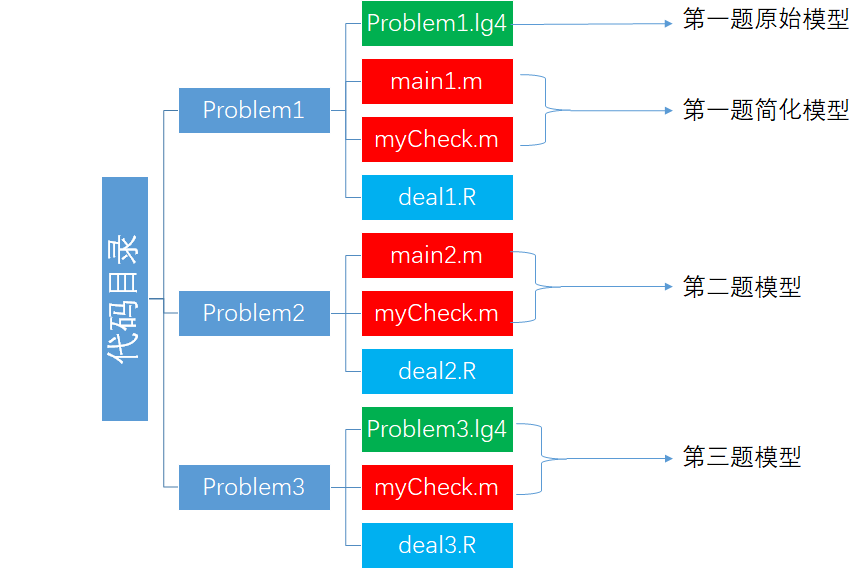
\includegraphics[width = 0.9\linewidth]{code.png}
			\caption{代码目录结构}
		\end{figure}
		
		\subsubsection{第一题代码}
		{
			我们在第一题有两个模型。原始模型代码用lingo撰写,简化模型代码由MATLAB撰写。两个模型代码可以分别单独运行。
			
			lingo代码见Problem1.lg4。注意需要有教育版(或完整版)lingo,试用版由于约束太多无法运行。
			
			简化模型代码如下:
			
			\begin{lstlisting}
clear all;
clc;

% 约束1
p=[240,300,360,390,270,330];
A1=zeros(48,56);
A1temp=eye(7)+diag(-ones(1,6),1);
A1temp=A1temp(1:6,:);
A1=blkdiag(A1temp,A1temp,A1temp,A1temp,A1temp,A1temp,A1temp,A1temp);
b1=(-repmat(p,1,8)-3)';

% 约束2
A2=zeros(42,56);
for m=1:7
    for i=1:6
        row=6*(m-1)+i;
        index1=7*(m-1)+i+1;
        index2=7*(m)+i;
        A2(row,index1)=1;
        A2(row,index2)=-1;
    end
end
b2=-8 * ones(42,1);

% 约束3
A3=zeros(4,56);
A3(1,1)=1;
A3(2,7)=1;A3(2,36)=-1;
A3(3,14)=1;A3(3,43)=-1;
A3(4,21)=1;A3(4,50)=-1;
b3=[0,-11,-11,-11]';

A=[A1;A2;A3];
b=[b1;b2;b3];

m=zeros(56,1);m(56)=1;
options = optimoptions('intlinprog','Display','off');

tic
x=intlinprog(m,1:56,A,b,[],[],zeros(56,1),[],[],options);
% x=linprog(m,A,b,[],[],zeros(56,1));经过实验整数线性规划计算收敛更快
toc

xmid=reshape(x,7,8)';
xmid=xmid+66;
% R2 的矩阵可以单独检验是否满足非线性约束
% flag=myCheck(xmid);
% if(flag)
%     disp('符合机械手非线性约束')
% else
%     disp('不符合机械手非线性约束')
% end

% 补充机械手1的部分
result=zeros(8,11);
result(:,3:9)=xmid;
for n=1:8
    result(n,2)=result(n,3)-3;
    result(n,1)=result(n,2)-63;
    result(n,10)=result(n,9)+3;
    result(n,11)=result(n,10)+103;
end

% 检查机械手的非线性约束
flag=myCheck(result);
if(flag)
    disp('符合机械手非线性约束')
else
    disp('不符合机械手非线性约束')
end

final=result(88)+3;
disp(['总时间为 ',num2str(final),' 秒'])
disp(['调度方案为:'])
result
			\end{lstlisting}
			
			其中myCheck是用来检查是否满足机械手非线性约束的函数,核心部分如下:
			\begin{lstlisting}
for i=2:4
	for j=1:(i-1)
		if(x(m,s(i))<x(n,s(j)) && x(m,s(i))+3+T(s(i)+1,s(j))>x(n,s(j)))
			flag=0;
		end
		if(x(m,s(i))>x(n,s(j)) && x(m,s(i))<x(n,s(j))+3+T(s(j)+1,s(i)))
			flag=0;
		end
	end
end
for i=2:7
	for j=1:(i-1)
		if(x(m,t(i))<x(n,t(j)) && x(m,t(i))+3+T(t(i)+1,t(j))>x(n,t(j)))
			flag=0;
		end
		if(x(m,t(i))>x(n,t(j)) && x(m,t(i))<x(n,t(j))+3+T(t(j)+1,t(i)))
			flag=0;
		end
	end
end
			\end{lstlisting}
			
			运行时需保证myCheck.m和main1.m在一个目录下。
			
			需要额外指出的是,实际测试时发现MATLAB版本不同可能带来intlinprog的参数个数不一样(我的是R2017b professional,有10个参数,队友R2017a和R2015a academic,只有9个参数)。
			
			此时可以去掉一个“$[]$”即可,即:\mcode{x=intlinprog(m,1:56,A,b,[],[],zeros(56,1),[],options);}。
				
			第二题是类似的情况。
			
		}
	
		\subsubsection{第二题代码}
		{
			第二题代码由MATLAB撰写。代码如下:
			\begin{lstlisting}
clear all;clc;

p=[500,660,570];
T1=[0,1,3,5;
    6,0,2,4;
    4,5,0,2;
    2,3,5,0];
T2=[0,2,4,6;
    5,0,2,4;
    3,5,0,2;
    1,3,5,0];
T1(:,5)=T1(:,1);
T1(5,:)=T1(1,:);
T2(:,5)=T2(:,1);
T2(5,:)=T2(1,:);

% 约束1
A1=zeros(24,32);
A1temp=eye(4)+diag(-ones(1,3),1);
A1temp=A1temp(1:3,:);
A1=blkdiag(A1temp,A1temp,A1temp,A1temp,A1temp,A1temp,A1temp,A1temp);
temp=diag(T1,1);
b1temp1=p+temp(1:3)'+2;
temp=diag(T2,1);
b1temp2=p+temp(1:3)'+2;
b1temp=[b1temp1,b1temp2];
b1=(-repmat(b1temp,1,4))';

% 约束2
A2=zeros(18,32);
for m=1:6
    for i=1:3
        row=3*(m-1)+i;
        index1=4*(m-1)+i+1;
        index2=4*(m+1)+i;
        A2(row,index1)=1;
        A2(row,index2)=-1;
    end
end
b2temp1=zeros(3,1);
for i=1:3
    b2temp1(i)=2+T1(i+1,i+2)+T1(i+2,i);
end
b2temp2=zeros(3,1);
for i=1:3
    b2temp2(i)=2+T2(i+1,i+2)+T2(i+2,i);
end
b2temp=[b2temp1;b2temp2];
b2=(-repmat(b2temp,3,1));

A3=zeros(9,32);
for m=1:7
    index1=4*(m-1)+1;
    index2=4*m+1;
    A3(m,index1)=1;
    A3(m,index2)=-1;
end
A3(8,1)=1;
A3(9,8)=1;A3(9,25)=-1;
b3=[-68,-68,-68,-68,-68,-68,-68,0,-114]';

A=[A1;A2;A3];
b=[b1;b2;b3];
m=zeros(32,1);m(32)=1;
options = optimoptions('intlinprog','Display','off');

tic

x=intlinprog(m,1:32,A,b,[],[],zeros(32,1),[],[],options);
%x=linprog(m,A,b,[],[],zeros(32,1));

xmid=reshape(x,4,8)';
xmid=xmid+66;

% 补充机械手1部分
result=zeros(8,8);
result(:,3:6)=xmid;
for n=1:8
    result(n,2)=result(n,3)-3;
    result(n,1)=result(n,2)-63;
    if((mod(n,2))==1)
        result(n,7)=result(n,6)+T1(4,5)+2;
    else
        result(n,7)=result(n,6)+T2(4,5)+2;
    end
    if(n>1 && result(n,7)<result(n-1,8)+5)
        result(n,7)=result(n-1,8)+5;
    end
    result(n,8)=result(n,7)+103;
end

toc

flag=myCheck(result);
if(flag)
    disp('符合机械手非线性约束')
else
    disp('不符合机械手非线性约束')
end


final=result(64)+3;
disp(['总时间为 ',num2str(final),' 秒'])
disp(['调度方案为:'])
result

			\end{lstlisting}
			
			其中myCheck是用来检查是否满足机械手非线性约束的函数,核心部分如下:
			
			\begin{lstlisting}
% 检查机械手2的约束
flag2=1;
temp2=zeros(1,length(mh2)-1);
for i=1:(length(mh2)-1)
	temp2(i)=T(room2(i),roomNext2(i))+2+T(roomNext2(i),room2(i+1));
	if((mh2(i+1)-mh2(i))<temp2(i))
		flag2=0;
	end
end

% 检查机械手1的约束
flag1=1;
temp1=zeros(1,length(mh1)-1);
for i=1:(length(mh1)-1)
	temp1(i)=T(room1(i),room1(i)+1)+2+T(room1(i)+1,room1(i+1));
	if((mh1(i+1)-mh1(i))<temp1(i))
		flag1=0;
	end
end
			\end{lstlisting}
			
			运行时需保证myCheck.m(注意不要错误地使用第一题的myCheck.m,两者不一样)和main2.m在一个目录下。
		}
	
		\subsubsection{第三题代码}
		{
			第三题代码由lingo和MATLAB共同编写。运行时先运行lingo,将结果保存成xlsx(88*1,名称命名为temp.xlsx)。然后MATLAB程序读取并检验。
		}
		\subsubsection{将结果转化为机械手的动作序列代码}
		{
			这一部分代码由R编写,使得我们得出的矩阵结果(8*11)能转化为题目要求的动作序列。
			见目录下deal1.R, deal2.R和deal3.R。
			
			运行时需要实现使用MATLAB \mcode{dlmwrite} 将结果保存成result.txt,然后再调用R将其转化为tex可读的表格格式。这一部分代码不是题目主要代码,可以不运行。
		}
    }

    \subsection{各成员的贡献}
    {
        最初,我们对于决策变量的选择,有两种方案的争论。
        一种是3人共同提出的,以8*11的时刻矩阵作为决策变量,这样目标函数很直观,而约束则较为复杂。
        另一种是尹秋阳提出的,以机械手的动作序列的顺序为决策变量。由于序列顺序唯一决定了系统的状态,因此是可行的。但是这是离散的决策变量,属于组合优化的范畴,我们参考组合优化的书籍简单讨论后,决定放弃这种方案。

        之后,金帆想出了有关机械手的不冲突的约束的表示方法,并用数学公式严格表述了出来,这就是本文中第一题的“原始优化模型”。之后,金帆对其做了少量简化(“等价的简化约束条件”),在LINGO中编写程序,实现了这个优化模型,计算耗时31秒。

        由于计算复杂度高,尹秋阳和李皓冉经过讨论,发现金帆的模型中的大部分非线性约束是不起作用的。因此,尹秋阳根据“引理1”,提出了“算法1”,通过减约束、忽略第一个机械手的方式,将问题转化为了简单的线性规划问题。决策变量个数从88下降到56个,约束个数从2000多个下降到了93个。最后模型求解时间大幅缩减到了0.3秒。在这个过程中,李皓冉完成了忽略机械手1可行性的证明,尹秋阳完成了其余部分的建模与代码编写。

        尹秋阳将金帆的第一题思路推广到了第二题,并提出了“加约束”的办法,依据引理2,通过第二题所述的“3个步骤”,得到了第二题的答案。事实上,这是一个从特殊到一般的过程。这3个步骤中,尹秋阳先求解出了一个4038的可行解,进而完成了第二步“交替”条件下最优性的证明;李皓冉补充证明了第三步的合理性,从而共同证明了答案的最优性,完成了第二问。

        李皓冉将第一题的思路推广到第三题,修改了第一题的原始模型使之能解决第三题的问题。他提出了废除元件进入次序的做法,依据引理1,依据算法1,在LINGO中得到了第三题的答案。尹秋阳编写了检查器检验得出结果的可行性。

        尹秋阳最后写了能将三小题的结果其转化为机械手的动作序列的代码。
        
        本报告主要由金帆撰写,题目中改进的模型和相应的数学证明部分由尹秋阳和李皓冉各自写出。
        
        回头来看,尽管我们早就得出了答案,但是相应的证明却卡了我们很久。为了逻辑的严谨性和得出结论的科学性,我们还是一步步得完成了解的最优性。
        
        总得来说我们团队比较融洽,每个人分工明确,相互协作。每个成员的贡献都很大,没有一个人是“挂机划水”的。希望助教评分时予以考虑。

    }
}

\clearpage
\end{document}
